\documentclass[12pt, a4paper]{article}
\usepackage{scrextend}
\usepackage{titlesec}
\usepackage{graphicx}
\usepackage{amsmath}
\usepackage{amsfonts} % for the real number symbol
\usepackage{geometry}
\usepackage[unicode]{hyperref}
\usepackage{titlesec}
\usepackage{titletoc}
\usepackage[sorting=none]{biblatex}
\usepackage{xurl}
\usepackage{enumitem}
\usepackage{indentfirst}
\numberwithin{equation}{section} % number equations by section
\renewcommand{\figurename}{Att.}
\renewcommand{\contentsname}{Saturs}
\renewcommand{\labelenumi}{\arabic{enumi})} % lists with 1)
\setlist{nosep}
\parindent=1cm
\linespread{1.213} % equivalent to 1.5 in word, experimentally.
\addbibresource{refs.bib}

\geometry{
    a4paper,
    lmargin=30mm,
    rmargin=20mm,
    tmargin=20mm,
    bmargin=20mm
}


\titleformat{\section}
    {\normalfont\large\bfseries}{\thesection . }{0.2em}{\MakeUppercase}
\titleformat{\subsection}
    {\normalfont\large\bfseries}{\thesubsection . }{0.2em}{}
\titleformat{\subsubsection}
    {\normalfont\normalsize\bfseries\itshape}{\thesubsubsection . }{0.2em}{}
\titlespacing*{\subsubsection}{0pt}{6pt}{0pt}

\begin{document}
\begin{titlepage}
    \begin{center}
        \vspace*{3cm}
        
        LATVIJAS UNIVERSITĀTE

        DATORIKAS FAKULTĀTE

        \vspace*{4cm}

        \large\textbf{ATDARINOŠĀS MAŠĪNMĀCĪŠANĀS PIELIETOJUMS ROBOTIKĀ}
        
        \vspace{2cm}
        \normalsize{MAĢISTRA KURSA DARBS}
         
             
    \end{center}
    \vspace{3cm}
    \begin{addmargin}[18em]{0em}
    Autors: \textbf{Pēteris Račinskis}
    \end{addmargin}

    \begin{addmargin}[18em]{0em}
    \hspace{1cm} Stud. apl. Nr. pr20015
    \end{addmargin}

    \begin{addmargin}[18em]{0em}
    Darba vadītājs: Dr. sc. comp. Modris Greitāns
    \end{addmargin}
         
    \vfill
    \begin{center}
    RĪGA 2022
    \end{center}
 \end{titlepage}
\newpage
\tableofcontents
\thispagestyle{empty}
\newpage
\setcounter{page}{3}


\section{Ievads}

Mašīnmācīšanās šobrīd tiek plaši uzskatīta par vienu no aktuālākajām datorzinātņu pētniecības nozarēm \cite{no_shit}. Pēdējās desmitgades laikā šī pētniecības lauciņa popularitāte ir daudzkārt pieaugusi, pateicoties galvenokārt diviem faktoriem: ļoti vispārīgiem neironu tīklu modeļiem un skaitļošanas resursu veiktspējai, kas beidzot ļāvusi šos teorētiski jau ļoti sen \cite{mcculloch1943logical, linnainmaa1970representation, fukushima1988neocognitron} iedomātos mākslīgā intelekta uzbūves elementus realizēt praksē. Tā risināti uzdevumi, ko izsenis daudzi uzskatījuši par neiespējamiem, un lietojuši kā argumentu pret mašīnmācīšanos kā rīku, kas spētu konkurēt ar bioloģiskas izcelsmes prātiem --- semantiskas nozīmes meklēšana attēlos \cite{krizhevsky2012imagenet}, tekstu korpusu analīze un ģenerēšana ar "izpratni" par to saturu \cite{vaswani2017attention} un visspējīgāko spēlētāju pārspēšana nepilnīgas informācijas spēlēs ar neaptverami milzīgiem iespējamo stāvokļu permutāciju skaitem \cite{silver2016mastering}.

Nav arī īpaši grūti atrast vēsturisko saikni starp mākslīgo intelektu un robotiku. Tautas iztēlē termins ``robots'' drīzāk droši vien iezīmēs zinātniskās fantastikas radītos personāžus --- mehāniskas būtnes, kas spēj patstāvīgi darboties neierobežotā vidē un risināt sarežģītus uzdevumus --- nevis pieticīgākus, reāli pastāvošus un ražotnēs rodamus industriālos robotus. Un šī pati zinātniskā fantastika radījusi arī nesaraujamu saiti starp robotiem un mākslīgo intelektu \cite{asimov2004robot} --- diskusijas par mākslīgo intelektu bieži plūstoši pāriet diskusijās par ar šādu intelektu aprīkotiem robotiem, un šo robotu neizbēgami kareivīgajām ambīcijām attiecībā pret cilvēci. Protams, zinātne ne vienmēr seko populār-zinātniskās iedomas lidojumam, taču šāda saikne ir visnotaļ pamatota --- spēja mācīties no paraugiem vai patstāvīgi un pielāgoties savai apkārtnei ir ārkārtīgi noderīga, jo daudzi uzdevumi, kuru risināšanai varētu pielietot robotus, ir sarežģīti nevis to fizikālajā izpildē, bet tieši vadības uzdevuma formulēšanā un realizācijā --- lai to redzētu pietiek vien aplūkot kādu nejauši izvēlētu sarakstu ar robotikā aktuālām problēmām \cite{popsci}.

Atdarinošā mašīnmācīšanās (\textit{imitation learning}) ir viens no paņēmieniem, ar kuriem tiek mēģināts risināt šādas sarežģītas vadības problēmas. Lai gan pamatu pamatos nevar apgalvot, ka tā ir tikai robotikai piemērota metožu saime, lielākā daļa izpētes virzīta tieši šajā virzienā --- problēmas tiek formulētas kā fizikālu (vai nosacīti fizikālu --- virtuālās vidēs simulētu) procesu kontroles uzdevumi, un risinājumi tiek rasti no pēc iespējas mazāka skaita veiksmīgas darbības piemēru \cite{attia2018global}. Mašīnmācīšanās nozarē bioloģiskas analoģijas un iedvesma nav nekāds retums, un savā ziņā šāda mācīšanās  atspoguļo vienu no izplatītiem paņēmieniem, kā cilvēki vai sabiedriski dzīvnieki nodod prasmes viens otram - demonstrējot. Nevar nepieminēt, ka izpēte šajā jomā bieži aizņemas pieejas un iespaidojas no rezultātiem, kas gūti ar stimulēto mašīnmācīšanos (\textit{reinforcement learning}) - savā ziņā vispārīgu, pašmācībai un treniņam analoģisku paņēmienu. Arī abu metožu apvienojums ir ideja, kas pavīd visai regulāri --- cerībā, ka, atdarinot ekspertus, var ātrāk nonākt pie derīgām stratēģijām, kas var kalpot kā sākumpunkts dziļākai pašmācībai \cite{hester2018deep}; vai arī izmantot šādu stimulēto metodi, lai precīzāk imitētu treniņa datus \cite{abbeel2004apprenticeship}.


\subsection{Darba mērķis un struktūra}

Šis ir maģistra kursa darbs --- pirmais konkrētais rezultāts, kas sasniegts maģistra darba izstrādes procesā. Tātad saturs un formāts ir lielā mērā atkarīgs no nākamajā semestrī aizstāvamā gala darba izstrādei individuāli nospraustajiem mērķiem un iztecējušā semestra gaitā reāli paveiktā. 

Kopējā maģistra darba tēma izvēlēta ar Elektronikas un datorzinātņu centra eks-pertu palīdzību, meklējot šobrīd aktuālu pētniecības virzienu. Izvērtējot dažādus pieejamos variantus, izvēlēts pētniecības virziens --- atdarinošā mašīnmācīšanās --- un konkrēts motivējošais uzdevums --- atkritumu šķirošanas līnijas robots, kas spēj nogādāt pudeles vai citus objektus tiem atbilstošajās tvertnēs, izmantojot mešanas kustības. Faktiski līdz šim galvenokārt veikta nozares literatūras avotu izpēte un nepieciešamo pamatzināšanu apguve. Līdz ar to šī darba mērķis ir noskaidrot, vai atdarinošās mācīšanās metodes ir piemērotas motivējošās problēmas risināšanai, atrast piemērotākos paņēmienus un aktuā-lākos rezultātus jau eksistējošajā zinātniskās literatūras korpusā un ieskicēt risinājuma plānu, kura praktiska izpilde un novērtēšana tad arī veidotu galadarba pētniecisko jaunpienesumu. Attiecīgi, kursadarbs sastāv no trijām daļām:
\begin{enumerate}
    \item ievada, kurā īsi izklāstīti vispārīgi jēdzieni, kas nepieciešami, lai izprastu zinātnisko literatūru nozarē, kā arī aprakstīts motivējošais uzdevums;
    \item literatūras analīzes, kur izdalīti daži galvenie pētnieciskās darbības virzieni nozarē, aplūkoti konkrēti algoritmi un pētījumi kā piemēri;
    \item secinājumiem, kur literatūras analīzē gūtās atziņas īsi apkopotas un izmantotas, lai piedāvātu provizorisku formu motivējošā uzdevuma risinājumam.
\end{enumerate}


\subsection{Terminoloģijas tulkojumi, apzīmējumi, saīsinājumi}

Viena no īpatnībām, ar ko ir nācies saskarties, strādājot tieši ar mašīnmācīšanās nozari, ir nepārprotamas terminoloģijas trūkums latviešu valodā. Pati zinātnes nozare, lai arī nebūt ne tik jauna kopumā, piedzīvojusi milzīgas izmaiņas un nepieredzētu uzplaukumu pēdējās desmitgades laikā. Protams, datorzinātnes laukā pirmā un galvenā saziņas valoda ir angļu. Attiecīgi novērajami divējādi un saistīti fenomeni - publikācijas un terminoloģija, kas radītas senāk, veidojušas dziļi specifisku nišu, kas nav iedvesmojusi daudz mēģinājumu tulkot to uz citām valodām, savukārt uzplaukuma laikos vēl ir ļoti daudz materiāla, ko vienkārši neviens nav paguvis iztulkot.

Patvaļīgi izvēloties tulkojumu, pastāv risks mulsināt lasītāju un sadrumstalot jau tā nelielo literatūras kopu dažādu atslēgas vārdu izvēles rezultātā. Kur vien iespējams, ieteicams izmantot oficiālā terminu datubāzē pieejamus tulkojumus, taču ne vienmēr tādi ir pieejami. Tāpēc šeit izveidots saraksts ar potenciāli mulsinoši tulkoto terminoloģiju tās oriģinālajā formulējumā angļu valodā, izvēlētajiem tulkojumiem un īsiem pamatojumiem.  

\begin{enumerate}
    \item \textit{policy} --- \textbf{stratēģija}. Šis termins pamatā tiek lietots, lai aprasktītu kādu funkciju, kas novērojumus attēlo lēmumu telpā. Pirmais ieraksts tieši tāpēc, ka varētu būt strīdīgākais. Angļu valodā pastāv divi termini, \textit{policy} un \textit{politics}, kas parasti latviski tiek tulkoti vienādi --- politika --- par spīti radikāli atšķirīgām nozīmēm. Termins \textit{strategy} tiek lietots kā sinonīms pirmajam abās valodās, un arī piemērojams tieši šādām lēmumu pieņemšanas funkcijām, piemēram, spēļu teorijā.
    \item \textit{reinforcement learning} --- \textbf{stimulētā mašīnmācīšanās}. Meklējumi tiešsaistē atklāj \cite{enc_stim}, ka šis tulkojums jau ir apstiprināts standartā, taču varētu būt nezināms lasī-tājiem, kas ar to sastopas pirmo reizi --- pat ja zināms metodes angliskais nosaukums.
    \item \textit{imitation learning} --- \textbf{atdarinošā mašīnmācīšanās}. Paša autora piedāvāts tulkojums, izmantojot iepriekšējo kā piemēru, jo nav izdevies atrast alternatīvas. Latvis-kais vārds "atdarināt" izvēlēts pār internacionālismu ``imitēt'', jo to vieglāk izlocīt formā, kas neizklausās lauzīta un neveikla. Taču procesā zūd spēja viegli atrast sākotnējo vārdu svešvalodā, kas ļoti svarīga zinātniskajā vidē, kurā latviski pie-ejamo resursu ir maz.
    \item \textit{reward function} --- \textbf{atalgojuma funkcija}. Oficiālā terminu datubāzē tulkojuma šim terminam nav. Tuvākie tulkojumi lietojumam, ar kādu šis termins parasti sastopams tekstos angļu valodā, būtu ``lietderība'' vai ``atdeve'', taču ``atalgojums'' labi ietver sevī faktu, ka šo funkciju paredzēts maksimizēt.
    \item \textit{generative adversarial network} --- \textbf{ģeneratīvie pretinieku tīkli}. Šim terminam arī pastāv vairāki konkurējoši tulkojumi, un terminu datubāzē skaidru atbildi nevar rast. Taču ir atrodams jau 2019. gadā sagatavotais kolēģes Lianas Blumbergas kursa darba plakāts, kur šis tulkojums ir lietots \cite{GAN}, tāpēc tas pats tiks lietots arī šeit.
\end{enumerate}

Tekstā var bez paskaidrojuma tikt izmantoti šādi saīsinājumi:

\begin{enumerate}
    \item RL --- stimulētā mašīnmācīšanās (\textit{Reinforcement Learning})
    \item IRL --- inversā stimulētā mašīnmācīšanās (\textit{Inverse Reinforcement Learning})
    \item GAN --- ģeneratīvais pretinieku tīkls (\textit{Generative Adversarial Network})
    \item VR --- virtuālā realitāte
    \item MDP --- Markova lēmumu process (\textit{Markov Decision Process})
    \item EDI --- Elektronikas un datorzinātņu institūts
    \item LIDAR --- attāluma lāzermērīšana
\end{enumerate}

Biežāk izmantoti matemātiskie apzīmējumi:

\begin{enumerate}
    \item $\pi, \pi_{\theta}, \pi^*$ --- stratēģija, stratēģija ar parametriem $\theta$, instruktora stratēģija
    \item $s$ --- sistēmas stāvoklis vai tiešais novērojums
    \item $s_t, s'$ --- $s$ laika solī $t$, nākamais $s$
    \item $a, a_t$ --- darbība, darbība laika solī $t$
    \item $o_t$ --- netiešais novērojums
    \item trajektorija --- laikrinda ar elementiem $s_t$, $o_t$, $(s_t, a_t)$ vai $(o_t, a_t)$, ja nav norādīts
    \item $R(s), R(s,a)$ --- atalgojuma funkcija
    \item $\theta, \phi, \psi$ --- modeļu parametru vektori
    \item $\mathbb{E}$ --- matemātiskā cerība
\end{enumerate}



\subsection{Tehniskās priekšzināšanas, definīcijas}

Pētot un veidojot spriedumus par zinātnisko literatūru viens no lielākajiem šķēršļiem lasītājam ``no malas'' ir katrā nozarē pieņemtais tehnisko priekšzināšanu kopums, ko autori sagaida no auditorijas. Tas, protams, ir loģiski, jo publikācija, kas apraksta jaunākos atklājumus kādā dziļi specifiskā lauciņā, nevar veltīt visu sev atvēlēto drukas apjomu elementāras un vispārzināmas terminoloģijas skaidrojumiem. Tāpat, tālāk atskaitē iztirzājot šos rakstus, noderīgi ir ieviest tiem kopīgus apzīmējumus un definēt visus vienuviet. Tāpēc šajā ievada daļā tiek īsi aprakstīti jēdzieni, kas jāizprot, lai varētu veikt literatūras analīzi un izdarīt secinājumus.

\subsubsection{Parametriski modeļi, šabloni}

Viens no visplašāk izmantotajiem formālismiem datizraces un mašīnmācīšanās lau-kos ir parametriskais modelis. Pamatā tam ir ideja, ka nezināmu funkciju, kuras rezultātus vēlamies paredzēt, var aproksimēt ar citu funkciju jeb modeli:

\begin{equation} 
    M(x) \approx f(x)
\end{equation}

Protams, šādu modeļu varētu būt bezgalīgi daudz, un tie visi var atšķirties pēc tā, cik labi spēj paredzēt nezināmās funkcijas vērtības. Tāpēc modeļu meklēšanai parasti izmanto šablonus - funkcijas, kuru argumentā papildus ievades datiem ir brīvi maināmi un kopīgi (tātad "apmācāmi") parametri $\theta$:

\begin{equation} 
    \text{Meklē } \theta:M(x \vert \theta) = M_{\theta}(x)  \approx f(x)
\end{equation}

Iegūtā šablona funkcijas un apmācīto parametru kombinācija $\lbrace M, \theta \rbrace$ tad veido konk-rētu modeli. Labs šablons ir tāds, kas spēj pielāgoties ļoti daudzām dažādām funkcijām:

\begin{equation} 
    \forall f \forall x \exists \theta:M_{\theta}(x)\approx f(x)
\end{equation}

Atkarībā no uzdevuma specifikas, izplatīti modeļi mēdz būt regresori, kas aproksimē funkcijas ar $k$-dimensionālām reālām (vai citādi skaitliskām) vērtībām,

\begin{equation} 
    f:x \rightarrow \mathbb{R}^k
\end{equation}
\begin{equation} 
    M: x \times \theta \rightarrow \mathbb{R}^k
\end{equation}

un klasifikatori, kas paredz ievades datu punkta piederību kādai diskrētai klasei

\begin{equation} 
    f:x \rightarrow C = \lbrace c_1, c_2, ..., c_m \rbrace
\end{equation}
\begin{equation} 
     M: x \times \theta \rightarrow C
\end{equation}

Bieži vien noderīgi ir ne tikai spēt attēlot datu punktu kā diskrētu klasi, bet iegūt varbūtību sadalījumu, kas apraksta tā iespējamību piederēt jebkurai no klasēm:

\begin{equation} 
    M: x \times \theta \times c_i \rightarrow [0; 1]
\end{equation}
\begin{equation} 
    M_{\theta}(x, c_i) = P_i
\end{equation}
\begin{equation} 
    \sum_{i=1}^m P_i = 1
\end{equation}

Lai varētu novērtēt, cik labi modelis aproksimē nezināmo funkciju, un vadīt parame-tru apmācības procesu, tiek izmantotas mērķa funkcijas (\textit{loss functions}) \cite{notation}:

\begin{equation} 
    \ell: M_{\theta}(x) \times f(x) \rightarrow \mathbb{R}
\end{equation}

Strādājot ar reāliem datiem, datu punkti veido datu kopu, kas parasti tiek uzskatīta par gadījuma izlasi no punktus ģenerējošā varbūtību sadalījuma. Praktiskiem apmācības uzdevumiem datu kopa parasti jāiegūst formā, kas satur gan sagaidāmos ievades datus, gan pareizu rezultātu:

\begin{equation} 
    s \sim \mathcal{D} \Leftrightarrow s \text{ ir no varbūtību sadalījuma } \mathcal{D}
\end{equation}
\begin{equation} 
    y_i = f(x_i)
\end{equation}
\begin{equation} 
    s_i = (x_i, y_i)
\end{equation}
\begin{equation} 
    S = \lbrace s_1, s_2, ..., s_n \vert s_i \sim \mathcal{D}\rbrace
\end{equation}

Datu kopai var aprēķināt empīrisku mērķa funkcijas novērtējumu,

\begin{equation} 
    L_S(\theta) = \frac{1}{n}\sum_{i=1}^n\ell(M_{\theta}(x_i), y_i)
\end{equation}

bet apmācības process parasti kādā veidā tiecas minimizēt šīs vērtības matemātisko cerību ģenerējošam sadalījumam (nevis tikai pašai datu kopai - ja modelis ļoti cieši pielāgots konkrētai datu izlasei bet zaudē precizitāti sadalījumam kopumā, to sauc par pārpielāgošanos --- \textit{overfitting})

\begin{equation} 
    L_{\mathcal{D}}(\theta) = \mathbb{E}_{\mathcal{D}} [\ell(M_{\theta}(x_i), y_i)]
\end{equation}
\begin{equation} 
    \text{Apmāca } M_{\theta} \text{ uz } \mathcal{D} \rightarrow \text{Minimizē } L_{\mathcal{D}}(\theta)
\end{equation}

Ja modelis ir stratēģija (\textit{policy}), stimulētās vai atdarinošās mašīnmācīšanās literatūrā to ļoti bieži izsaka kā $\pi_{\theta}(x)$. Mazliet mulsinošs ir tieši ar imitējošām metodēm saistītos rakstos lietotais apzīmējums $\pi^*$, ar ko apzīmē t.s. ``ekspertu stratēģijas'' --- kas pašas ir nezināmās funkcijas, ko cenšamies aproksimēt pēc to ģenerēto punktu kopām. 


\subsubsection{Neironu tīkli}

Neironu tīkli ir izplatīta modeļu šablonu saime, ko var izmantot dažādas formas funkciju aproksimēšanai --- tie var būt gan klasifikatori, gan regresori. Neironu tīklu kopīgais elements ir t.s. perceptorns, kas izteikts jau pašos pirmsākumos \cite{mcculloch1943logical}. Perceptrons funkcija, kas piemēro nelineāru aktviācijas funkciju $\sigma$ argumentu vektora $\vec{x}$ elementu savstarpējai lineārai kombinācijai, t.i,


\begin{equation} 
    f_{perceptron}(\vec{x}) = \sigma(\vec{w} \cdot \vec{x}+b)
\end{equation}

kur $\vec{w}$ ir t.s. svaru vektors, bet $b$ ---  nobīde. Perceptrona parametri tātad ir brīvie mainīgie $\vec{w}$ un $b$. Neironu tīkls parasti sastāv no slāņiem --- perceptronu $f_i$ kopām, kas visi apstrādā to pašu argumentu vektoru, bet katrs ar saviem parametriem $\vec{w}_i,b_i$. Tad slāni algebriski izsaka formā

\begin{equation} 
    W = \begin{bmatrix}
        w_1^T \\
        w_2^T \\
        ... \\
        w_k^T
    \end{bmatrix}; 
    \vec{b} =  \begin{bmatrix}
        b_1 \\
        b_2 \\
        ... \\
        b_k
    \end{bmatrix}; 
\end{equation}
\begin{equation} 
    f_{layer}(\vec{x}) = \sigma(W\vec{x}+\vec{b})
\end{equation}

Ja slānis tīklā ir pēdējais un tā vērtības ir modeļa izvadē, to sauc par izvades (\textit{output}) slāni. Ievades datu vektoru sauc par ievades (\textit{input}) slāni. Pārējos slāņus sauc par slēptajiem (\textit{hidden layers}). Saka, ka slāņi savā starpā pilnīgi savienoti (\textit{fully connected}), ja katram viena slāņa perceptronam argumentā parādās visi iepriekšējā slāņa izvades elementi. Svarīga neironu tīkla īpašība --- ja tā aktivācijas funkcijas ir diferencējamas, tad arī tīkls kopumā ir diferencējams pēc katra tā parametra, pat ar perceptroniem daudzos slāņos. Līdz ar to var izmantot t.s. \textit{backpropagation} algoritmu, kas atrod mērķa funkcijas parciālos atvasinājumus pēc modeļa parametriem un izmanto kādu gradientu optimizācijas metodi apmācībai.

Pastāv dažādas šo tīklu arhitektūras. Vienkāršākās sastāv no viena vai vairākiem slāņiem (neskaitot ievades slāni), taču ir plaši izplatīti arī, piemēram, konvolūciju neironu tīkli \cite{krizhevsky2012imagenet}, ko izmanto attēlu apstrādē, tai skaitā šajā atskaitē aplūkotajos pētījumos, kur nepieciešams gūt informāciju no video datiem. Galvenā atšķirība konvolūcijā tīklā ir kodola funkciju (\textit{kernel}) izmantošana - konvolūciju slāņi vienā līmenī piemēro identiskas perceptrona funkcijas nelieliem iepriekšējā slāņa (matricas vai tenzora formā) reģioniem. Tas palīdz identificēt dažādas lokālas struktūras, piemēram, attēlā. Šo un vēl citu veidu sarežģītāku neironu tīklu arhitektūra ir ļoti plašs lauks, ko detalizēti šeit iztirzāt nav iespējams.

\subsubsection{Markova lēmumu procesi}

Pastāv dažādi formālismi procesu definēšanai vadības sistēmu izstrādes mērķiem, lai ar tiem varētu veikt matemātiskas operācijas. Izplatīti atdarinošās un stimulētās mašīnmācīšanās literatūrā ir Markova lēmumu procesi (MDP --- \textit{Markov decision processes}), kas izmantojami situācijās, kad sistēmas stāvokli nākotnē pilnībā nosaka pašreizē-jais. Dažādi autori, kas darbojas dažādos izpētes virzienos, mēdz piedāvāt dažādus tā formulējumus, taču parasti tie ir ekvivalenti sekojošam \cite{attia2018global}

\begin{equation} 
    MDP = (S,A,R,T, \gamma)
\end{equation}

kur $S$ --- sistēmas iespējamo stāvokļu $s$ kopa; $A$ --- kontrolētajam procesam (``aģen-tam'') pieejamo darbību $a$ kopa; $R: S \times A \rightarrow \mathbb{R}$ vai $R: S \rightarrow \mathbb{R}$--- atalgojuma (\textit{reward}) funkcija, kas ļauj kārtot sasniegtos stāvokļus pēc to tīkamības; $T: S \times A \rightarrow S$ vai $P(s' \in S)$ --- pārejas (\textit{transition}) funkcija, kas nosaka nākamo stāvokli $s'$ vai tam atbilstošu varbūtību sadalījumu, ja pie iepriekšējā stāvokļa $s$ izvēlēta darbība $a$; $\gamma$ --- koeficients nākotnes atalgojumu vērtību samazināšanai. MDP ir \textit{galīgs} ja $S,A$ ir galīgas kopas. Ja $s' = T(s,a)$ ir determinēts, MDP ir \textit{determinēts}. Ja $s'$ ir gadījuma lielums, kas pieder sadalījumam $P(s')=T(s,a)$, MDP ir \textit{stohastisks}.

Atdarinošās mašīnmācīšanās metodēm ne vienmēr ir nepieciešams definēt atalgojuma funkciju un attiecīgi arī $\gamma$, taču tie ir nepieciešami metodēm, kas lieto stimulēto mašīn-mācīšanos. Tā kā parasti spriests tiek par stratēģijām $\pi_{\theta}$, kas izvēlas nākamo darbību $a$ atkarībā no sistēmas stāvokļa $s$, tad bieži vien faktiskā pārejas funkcija ir formā $P(s') = T(s, \pi_{\theta}(s), s')$, t.i., pārejas funkcija apraksta ``vides'' (\textit{environment}) reakciju uz aģenta (modeļa, stratēģijas) darbību. Pie sākotnējo stāvokļu kopas $S_0$ un stratēģijas $\pi$ var spriest par stratēģijas inducēto stāvokļu sadalījumu $s_t \sim P(S \vert S_0, \pi)$ --- tas nosaka, kādas trajektorijas vispār ir iespējamas pie šādiem nosacījumiem. 

Faktiski gandrīz nekad nav pieejams vides momentānā stāvokļa pilns raksturojums. Tā vietā zināma ir kāda to aprakstošu atribūtu apakškopa --- novērojums $o_t = g(s_t)$. Gadījumos, kad šie novērojumi veido vadības algoritma vajadzībām pietiekami precīzu un tieši pielāgojamu stāvokļa aprakstu, nekādi papildu formālismi nav nepieciešami --- tos var saukt par \textit{tiešiem novērojumiem} un uztvert kā ekvivalentus stāvokim $s_t$. Ja nepieciešami papildu soļi, lai no novērojuma iegūtu vadības algoritmam derīgu stāvokļa raksturojumu, tos sauc par \textit{netiešiem novērojumiem}.

Trajektoriju caur sistēmas stāvokļu (konfigurāciju) telpu, kādai process seko ar laika soļiem $t = \lbrace 1, 2, ..., T \rbrace$, var izteikt kā laikrindu formā, kas sastāv no \textit{state-action} pāriem --- $((s_1, a_1), (s_2, a_2), ..., (s_T, a_T))$. Ja šī laikrinda tiek izmantota kā paraugs treniņa procesā, to var saukt par demonstrāciju. Stāvokļus tajā, protams, iespējams aizstāt ar novērojumiem situācijās, kad tiek izmantota nepilnīga informācija. Ne viennmēr vēlams vai iespējams modelēt sistēmu ar MDP. Ir iespējami gadījumi, kad pārejas funkcija vai stratēģija ir atkarīga no laika soļa, kā arī sistēmas, kurās ar novērojumiem nepietiek lēmuma pieņemšanai un nepieciešams ņemt vērā iepriekšējo stāvokļu un darbību virkni, lai pareizi spriestu par slēptiem stāvokļa atribūtiem. 

\subsubsection{Stimulētā mašīnmācīšanās}

Stimulētā mašīnmācīšanās ir pati par sevi ļoti aktuāla izpētes nozare, un nereti nodarbojas ar to pašu vai līdzīgu uzdevumu risināšanu, kā atdarinošā. Pastāv ne tikai kombinēti paņēmieni \cite{gupta2019relay, brown2019extrapolating}, bet arī atdarināšanas metodes, kas tiešā veidā izmanto stimu-lēto mācīšanos, lai atdarinātu trajektoriju demonstrācijas \cite{englert2018learning}. Tāpēc nav nekāds pārstei-gums, ka šis termins visnotaļ bieži parādās ar atdarinošo mašīnmācīšanos saistītos pētīju-mos, citreiz bez nekādiem papildus paskaidrojumiem.

Stimulētās mašīnmācīšanās teorētiskie pamati ir galīgi MDP un Belmana vienādo-jums \cite{sutton2018reinforcement}. Pieņem, ka katram stāvoklim ir kāds atalgojums $R(s_t)$, bet uzdevums --- maksimizēt šo atalgojumu summu visā trajektorijas garumā $\sum_{t=1}^T R(s_t)$. Tad var izteikt arī varbūtību sadalījumu atalgojumam katram stāvokļa un darbības pārim

\begin{equation}
    p(s', r \vert s_t, a_t) = P[s_{t+1}=s', r=R(s')]
\end{equation}

Nākotnē sagaidāmās atalgojuma vērtības, ņemot vērā dilšanas koeficientu $\gamma$,  var izteikt kā

\begin{equation}
    G_t = \sum_{k=0}^{T-t} \gamma^k R(s_{t+k+1})
\end{equation}

Jebkura stratēģija katram stāvoklim nosaka darbību vai darbību sadalījumu $p(a \vert s) = \pi(a,s)$. Var izmantot rekursīvu sakarību, lai katram stāvoklim piekārtotu sagaidāmo atalgojumu jeb vērtību $v_{\pi}(s)$, kas atkarīga no izmantotās stratēģijas --- Belmana vienādojumu.

\begin{equation}
    v_{\pi}(s) = \mathbb{E}_{\pi}[G_t \vert s_t = s] = \sum_{a}\pi(a,s)\sum_{s', r}p(s', r \vert s_t, a_t)[r + \gamma v_{\pi}(s')]
\end{equation}

Atrisināt mācīšanās uzdevumu tādā gadījumā nozīmē atrast stratēģiju, kas maksimizē atalgojumu. Pastāv dažādas metodes, kā to darīt. Teorētiski vienkāršākais taču praktiskiem uzdevumiem reti piemērojams paņēmiens ir tā saucamā Q-mācīšanās. Tā strādā samērā vienkārši --- tiek izveidots tenzors $Q$ ar elementu, kas atbilst katrai iespē-jamai $(s,a)$ vērtībai, tam tiek piešķirta kāda sākotnējā vērtība (piemēram, 0). 

Apmācība notiek, izvēloties

\begin{equation}
    a_t = \operatorname*{argmax}_a Q(s_t = s, a)
\end{equation}

un sasniedzot trajektorijas beigas --- vai nu pēc noteikta soļu skaita $T$, vai arī kāda pārtraukšanas nosacījuma. Tad iegūtajai trajektorijai $(s_1, a_1), (s_2, a_2), ..., (s_T, a_T)$ no bei-gām aprēķinot $G_1, G_2, ... G_T$ atbilstoši katram solim var koriģēt vērtības tenzorā, kur $Q^i$ apzīmē tenzora vērtības i-tajā treniņa solī

\begin{equation}
    Q^{i+1}(s_t,a_t)=f(Q^{i}(s_t, a_t), G_t)
\end{equation}

Kaut gan šai metodei ir teorētiskas konverģences garantijas pēc pietiekama iterāciju skaita, ļoti strauji pieaug tās modeļa --- tenzora $Q$ --- parametru skaits, pieaugot iespējamo stāvokļu un darbību skaitam --- nepieciešams atsevišķi optimizēt katru iespējamo kombināciju, iespējams, ļoti daudzās iterācijās. Tāpēc praksē parasti tiek lietoti modeļi, kas aproksimē $v_{\pi}(s)$, piemēram, aģenta-kritiķa (\textit{actor-critic}) neironu tīkli, kas reizē iemācās paredzēt gan sagaidāmo vērtību, gan labāko darbību katram stāvoklim ar potenciāli daudz kompaktāku modeli.

Lai uzdevumu varētu risināt, nepieciešams spēt izteikt kādu analītisku funkciju, kas apraksta pašreizējā stāvokļa tīkamību --- izšķir labus rezultātus no sliktiem, vai starpstāvokļiem. Robotikā var būt sarežģīti šādu funkciju izdomāt, turklāt tā var būt ļoti ``retināta'' stāvokļu-darbību telpā, t.i., tikai ļoti nelielam skaitam (vai ar ļoti nelielu varbūtību) sasniegto stāvokļu atalgojuma funkcija $R(s_t)$ pieņem nenulles vērtību. Tieši šādu trūkumu mēģina risināt metodes, kas kombinē ekspertu demonstrāciju aproksi-mēšanu ar adaptīvu pielāgošanos \cite{nair2018overcoming}

\subsection{Motivējošais uzdevums}

Nevarētu apgalvot, ka atdarinosā mašīnmācīšanās kā tēma šim kursa darbam un maģistra darbam kopumā tikusi izvēlēta tīri inženiertehniskā procesa rezultātā --- sākot ar problēmas definīciju un nonākot pie tai piemērotākā risinājuma, pārbaudot un atsijājot visas iespējamās pieejas, priekšlaicīgi neieguldot pārāk daudz pūļu un resursu kādas konkrētas metodes pielietošanā. Daļēji orientē vēlme --- gan no EDI, gan autora puses --- izzināt jaunas kompetences un likt pamatu tālākiem pētījumiem. Tomēr vienu šobrīd aktuālu praktisku problēmu, kas šķiet piemērota tieši atdarinošās mašīnmācīšanās metodēm, var izteikt kā motivējošu uzdevumu. Bruņojoties ar šādu konkrētu mērķi, nozares literatūras pārskatu un teorētisko zināšanu apguvi iespējams strukturēt un prioritarizēt.

Situāciju var aprakstīt sekojoši. Atkritumu šķirošanas līnijas ir cilvēkam nedrau-dzīga un nepatīkama darba vide. Šobrīd tiek aktīvi meklēti veidi, kā palielināt to automatizācijas pakāpi --- gan izmaksu samazināšanas, gan darba drošības nolūkos \cite{trashbot}. Konkrēti aplūkojot plastmasas iepakojumu šķirošanu, jau izstrādātas metodes to klasifikācijai un satveršanai \cite{trashbot}. Viens no virzieniem, kurā varētu pilnveidot šo un citādu robustu, neregulāras formas objektu \textit{pick-and-place} uzdevumu risinājumus, ir metienu iestrādāšana trajektorijās. Ja pārvietojamais objekts ir noturīgs pret trieciena slodzēm vai tā stāvoklis nav svarīgs, un tā masa salīdzinot ar robota pašmasu ir neliela, potenciāli iespējams ievērojami paātrināt satveršanas un pārvietošanas ciklu laikus, jo nav nepieciešams visu robotu pārvietot līdz galamērķim. Turklāt paveras iespējas tieši šķirošanas uzdevumos, jo iespējams telpā brīvāk izvietot tvertnes, uz kurām objekti jānogādā --- metiens var nogādāt objektu tālāk, nekā maksimāli izstiepies robots. Protams, mēģinot manuāli programmēt katru metienu rodas virkne problēmu --- dažādi trajektoriju sākumpunkti, dažādi galamērķi un to iespējamā mainība, objektu neregularitāte, u.c. Tāpēc analītisku risinājumu atrast varētu būt ļoti nepraktiski, un tiek apsvērts mašīnmācīšanās metožu lietojums.

Attiecīgi var uzskaitīt šādus nosacījumus uzdevumam:
\begin{enumerate}
    \item var pieņemt, ka sākuma stāvoklī robots jau ir satvēris objektu, ja nepieciešams;
    \item trajektorijas sākumpunkti ir mainīgi --- jāspēj izdarīt metiens no dažādām pozīcijām;
    \item ir zināma objekta klasifikācija un līdz ar to --- tā vēlamais galamērķis;
    \item vēlamie galamērķi var būt dažādi un mainīgi;
    \item rezultējošo modeli jāspēj pielāgot apstākļiem darba vidē bez pārlieku darbietilpīgas un dārgas treniņa procedūras.
\end{enumerate}

Nav grūti redzēt, ka šādam uzdevumam par atalgojuma kritēriju pieņemot trāpīšanu pareizajā tvertnē, funkcijas vērtības būs ļoti retinātas, kas apgrūtina klasisko stimulētās metožu pielietojumu. Nākamās nodaļas ietvaros tiek veikts vispārīgs atdarinošās mašīn-mācīšanās metožu pētniecības pārskats, paturot prātā izvēlētā uzdevuma specifiku --- pievēršot uzmanību tiem rezultātiem un secinājumiem, kas varētu būt nozīmīgi problēmas risināšanā. Noslēgumā tiek izdarīti secinājumi par to, kuras citur gūtās atziņas ir svarī-gākās, un piedāvāts rīcības plāns motivējošā uzdevuma izpildei.

\newpage
\section{Literatūras analīze}

Šīs nodaļas mērķis ir izveidot aptuvenu nozares pētniecības saturisku pārskatu; aprakstīt galvenos sasniegtos rezultātus, gūtās atziņas katrā no tematiskajiem apakš-virzieniem. Protams, ne visus pētījumus iespējams vienkārši klasificēt pēc to piederības šeit izvēlētajām kategorijām, un daudzi varbūt tajā vispār neiederas --- taču cenšoties gūt personisku izpratni par kādu tēmu, lai motivētu tālākus pētījumus, ir svarīgi nostatīt iepriekšējus rezultātus to kontekstā. Saprast, kāpēc tieši šobrīd aktuālie pētniecības virzieni ir tādi, kādus tos varam redzēt kādā akadēmisko publikāciju datubāzē vai neseno pētījumu pārskatā.

Varētu sacīt, ka tieši par atdarinošo mašīnmāīšanos rakstīts ir samērā maz. Noteikti, ja salīdzina ar vispārīgākām metodēm vai rīkiem. Taču pat ``samērā maz'' tomēr nozīmē ļoti lielu publikāciju skaitu, kas apraksta pētījumus ļoti dažādos virzienos. Turklāt robo-tika dominē kā pielietojuma mērķis šādām metodēm. Lai radītu priekštatu par nozares pašreizējo stāvokli un tematisku dalījumu, nolemts izšķirt trīs aptuvenus virzienus, kas labi apraksta lielu daļu no pētījumiem par iespējām robotus apmācīt ar piemēriem:

\begin{enumerate}
    \item trajektoriju kopēšana --- mērķi šeit pamatā ir panākt robustu, precīzu atdarināšanu ar nelielām treniņa datu kopām, ja pieejama visa nepieciešamā informācija par sistēmas stāvokli;
    \item novērojumu iegūšana, interpretācija, papildināšana --- ne vienmēr ir pieejami dati padevīgā formā, lai tiešā veidā varētu imitēt tajos veiktās darbības. Daudzi pētījumi nodarbojas tieši ar apmācībai derīgu novērojumu iegūšanu --- netiešu (piemēram, video) novērojumu pārveidošanu, labākām cilvēka-robota saskarnes metodēm, trajektorijām ar nezināmām darbībām, u.c.;
    \item atdarināšana un adaptācija, vispārināšana --- atdarinošās mācīšanās pielietojums, lai uzlabotu stimulēto, un otrādi; vispārīgu prasmju iegūšana no demonstrācijām, tūlītēja atdarināšana. Kā panākt, ka neaprobežojamies ar tikai piemēros esošo un spējam pielāgoties? Kā efektīvi uzsākt stimulēto mācīšanos ļoti retinātās atalgojumu telpās?
\end{enumerate}

\subsection{Labi definētu trajektoriju kopēšana}

Pirmā, varētu teikt galvenā taču ne vienmēr vienkāršākā problēma, ir atrast veidu, kā piejamās ekspertu zināšanas --- robotikas kontekstā tās parasti būs pareizas trajektorijas dažādu pārvietojumu un smalku manpiulācijas uzdevumu risināšanai --- tiešā veidā atdarināt. Šo procesu mēdz saukt arī par programmēšanu ar demonstrācijām (PBD --- \textit{programming by demonstration}) \cite{muench1994robot,billard2008handbook}. Idealizētā vidē ar determinētām stāvokļu pārejām un pilnīgu informāciju par tās pašreizējo konfigurāciju šis uzdevums varētu būt pat triviāls, taču praksē saskaramies ar problēmām:

\begin{enumerate}
    \item darbs notiek ar novērojumiem, nevis stāvokļiem. Pat ja pieejami, piemēram, trajektoriju ieraksti, bieži vien trūkst svarīgas informācijas (varētu būt zināma trajektorijas kinemātika, bet ne tās dinamika --- paātrinājumi, bet ne spēki);
    \item atšķirības vidē: izpildelementos --- varbūt robots ir nedaudz citāds; apkārtnē --- varbūt manipulējamo objektu masas, forma vai izvietojums ir nedaudz atšķirīgi no demonstrācijās esošajiem;
    \item ja trajektoriju ģenerējis eksperts, kam, iespējams bijusi pieejama informācija, kuras aģentam nav --- piemēram, manipulāciju veicis cilvēks ar redzi, bet robotam pieejami tikai kontakta sensori.
\end{enumerate}

Problēmas faktiski nozīmē to, ka reālā sistēmā stāvokļu pārejas nav determinētas attiecībā pret novērojumiem un darbībām. Lai labāk saprastu šos trūkumus, vispirms noderīgi ir aplūkot ``naivākos'' veidus, kā varētu imitēt piemērus. Šajā apakšnodaļā aprakstīti pētījumi, kuros uzsvars ir uz pietiekami detalizētu demonstrāciju atdarināšanas procesiem.

\subsubsection{Vienkāršas metodes}

Pirmais, ko varētu darīt, ir tiešā veidā ierakstīt trajektoriju un to atkārtot. Šī nebūt nav jauna ideja --- gandrīz visiem mūsdienu industriāliem robotiem ir pieejamas t.s. \textit{lead-through} un \textit{teach-in} programmēšanas metodes, kas ļauj fiziski un ar tālvadības ierīces palīdzību vadīt robota kustību un to ierakstīt pēcākai atdarināšanai \cite{teach_pendant}, turklāt tās parādījušās jau pašos industriālās robotikas pirmsākumos 1970os gados \cite{abb2016special}.

Tā kā trajektorijai jābūt ierakstītai tieši ar robotu, lai tā būtu atkārtojama bez papildus datizraces uzdevumu risināšanas, var paredzēt, ka dabiski radīsies zināma tendence dominēt viegli realizējamiem bet varbūt ne optimāliem ceļiem telpā --- vieglāk ierakstīt dažus pagrieziena punktus un ļaut programmatūrai interpolēt nekā fiziski vadīt robotu visā kustības ceļā. Pie tam var parādīties neparedzēti trūkumi, pārejot no lēnas, nenoslogotas izpildes programmēšanas procesā uz ātru un noslogotu ekspluatācijā, kas apgrūtina procesu. Faktiski sākotnējais ieraksts bieži vien kalpo par starta punktu, bet, lai nonāktu pie lietojamas programmas, nepieciešams iegūto kodu koriģēt un iteratīvi pielāgot. Lai arī principā tiek izmantota demonstrācija trajektorijas iegūšanai, procesa veikšanai tik un tā nepieciešams personāls ar robotu programmēšanas prasmēm. Jau sen atzīts \cite{muench1994robot,billard2008handbook}, ka, lai tik tiešām robotus varētu apmācīt tikai ar piemēriem, nepieciešamas metodes, kas ir robustākas pret nobīdēm no paraugu ģenerējošā procesa apstākļiem un vispārināmākas, tāpēc uzsākti pētījumi ar mašīnmācīšanās metodēm.

Kad jāspēj atdarināt kas vairāk nekā viena, nemainīga trajektorija, nepieciešams atdarināt nevis pašu trajektoriju, bet gan procesu, kas tādas ģenerē --- ``eksperta'' jeb ``instruktora'' stratēģiju. Viena no vienkāršākajām metodēm, kas bieži tiek lietots kā piemērs, taču praksē reti kad ir pielietojuma, ir uzvedības klonēšana (\textit{behavioural cloning}). Vispārīgi to definēt ir samērā vienkārši \cite{attia2018global}. Ja dots MDP un kāda eksperta stratēģija $\pi^*$, kas šo MDP optimāli risina, mērķis ir atrast maksimāli tuvu modeli $\pi_{\theta}$, kur

\begin{equation}
    \pi_{\theta}(s) \approx \pi^*(s)
\end{equation}

Parasti, protams, ir pieejama datu kopa ar eksperta izietajām stāvokļu-darbību laikrindām, turklāt jāstrādā ir ar novērojumiem, nevis stāvokļiem. Lai veidotu vispārīgu izpratni par atdarinošo mašīnmācīšanos, noderīgi ir detalizētāk aplūkot kādu vienkāršu tās piemēru. Uzvedības klonēšana sistēmā, kur netiek veikta intensīva treniņa datu pārstrāde vai vadības algoritma argumentu pārveidošana ļoti labi kalpo šādiem mērķiem, tāpēc piemēram var izmantot 1989. gadā Kārnegija-Melona Universitātē veikto pētījumu ``\textit{Autonomous Land Vehicle in a Neural Network}'' (ALVINN) \cite{pomerleau1989alvinn}. Tā mērķis bija izstrādāt pašbraucošu automašīnu, kas spēj sekot ceļa kontūram.

Automašīna tikusi aprīkota ar videokameru un LIDAR sensoriem, kas devuši divus skatus uz to pašu telpas reģionu automobiļa priekšā. Par apmācāmo modeli izvēlēts neironu tīkls. Protams, 1989. gads vēl bija laiks, kad datoru veikstpēja bija stipri ierobežota, un nevienam vēl nebija ienācis prātā būvēt tik dziļas, daudzskaitlīgas un sarežģītas tīklu arhitektūras kā mūsdienu konvolūciju tīklus vai transformatorus. Tāpēc neironu tīkls ir gaužām līdzīgs jebkurā mācību grāmatā pirmajā nodaļā atrodamajiem piemēriem --- tam ir viens slēptais slānis ar 29 perceptroniem, kam seko 45 izvades elementi. Video izmantots krāsainā attēla zilais kanāls, jo tajā ceļa virsma visvairāk kontrastē ar apkārtējo vidi. Gan video, gan LIDAR radītie attēli tīkla ievadē veido vienkāršu vektoru bez nekādiem telpiskiem kodējumiem, visi slāņi savstarpēji pilnībā savienoti.

\begin{figure}[t!]
    \centering
    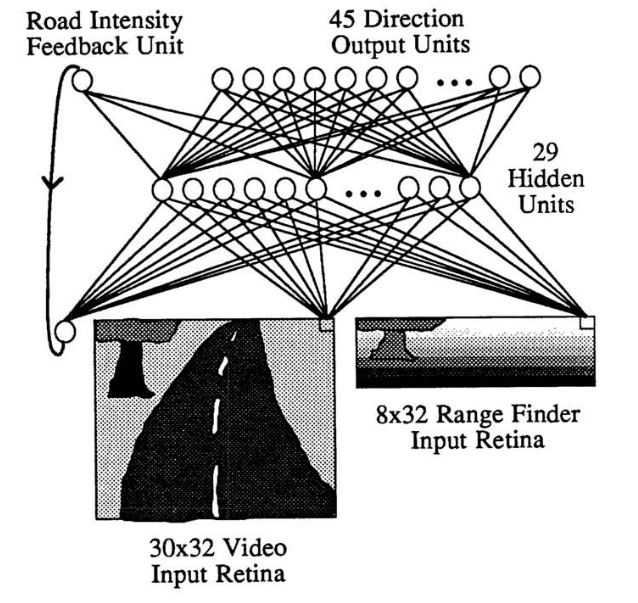
\includegraphics[height=6.8cm,page=1]{../img/alvinn_architecture.png}
    \caption{ALVINN modeļa uzbūve \cite{pomerleau1989alvinn}}
\end{figure}

Modeļa izvades slānis apzīmē vēlamo stūrēšanas virzienu 45 diskrētos soļos. Treniņa datu kopā faktisko virziena komandu atspoguļo neprecizēta veida ``zvana'' funkcija ar modu pie pareizā virziena. Ieviests viens papildus perceptrons, kas (teorētiski) novērtē ceļa gaišumu salīdzinot ar apkārtējo vidi, un tiek pievienots nākamās iterācijas ievades vektoram.

Jau šim (šķietami) samērā vienkāršajam uzdevumam konstatēts, ka ievākt treniņa datus fizikālā vidē --- braucot ar automašīnu pa ceļiem un ierakstot vadītāja veiktās korekcijas --- nav praktiski, jo nepieciešama ļoti liela treniņa datu kopa. Jāatzīst, ka ar modernākiem tehniskās redzes modeļiem droši vien šī nepieciešamība mazinātos. Tāpēc dati ģenerēti sintētiski --- tā kā gan video, gan attāluma datu izšķirtspēja ir gaužām neliela, pat ar 1989. gadā pieejamām datorgrafikas iespējām šādi gūtus attēlus ir grūti atšķirt no īstiem. Simulatorā iegūtie attēli un vadības komandas izmantoti klasifikatora apmācībā.

Iegūtais rezultāts --- modelis, kas maksimāli tuvināts simulatorā realizētajam kontroles algoritmam izmantotā šablona iespēju robežās. Tas bijis pietiekami labs, lai spētu vadīt ar kameru un attāluma sensoru aprīkotu automobili pa 400m garu slēgta ceļa posmu saulainos dienas apstākļos, ar ātrumu 0,5m/s. Tas tiek lietots kā arguments par neironu tīklu pavērtajām iespējām pašbraucošo auto attīstībā, taču netiek slēpts, ka sasniegtais ir tālu no praktiskas vadības sistēmas.

Kā galvenais uzvedības klonēšanas trūkums parasti tiek minēta nespēja atgūties no faktiskā stāvokļa sadalījumu nobīdes \cite{attia2018global} (\textit{distribution shift}). Ja reālais modelis $\pi_{\theta}(s)$ nevar pilnīgi precīzi atdarināt eksperta $\pi^*(s)$ darbības vai MDP pārejas funkcija ir stohastiska, tātad treniņa datu kopa neietver visas iespējamās trajektorijas ar atbilstošajām $\pi^*(s)$ vērtībām, $\pi_{\theta}$ inducētais stāvokļu sadalījums diverģē no $\pi^*$ inducētā. Lai iegūtu precīzāku un robustāku eksperta stratēģijas atdarinājumu, piedāvāti dažādi --- sarežģītāki --- apmācības paņēmieni.


\subsubsection{Statistiskas korekcijas}

Viens no virzieniem, kurā vesti centieni uzlabot trajektorju kopēšanas lietderību, ir strukturēt treniņa datu ieguvi un apmācības algoritmu veidā, kas maksimāli tuvina $\pi^*$ un $\pi_{\theta}$ inducētos stāvokļu sadalījumus. Bieži vien tas nozīmē, ka vienkārši ievākt datus un veikt apmācību uz tiem vairs nav iespējams --- nepieciešama aktīva instruktora iesaiste. Piedāvātie risinājumi ir dažādi, un metodes var kļūt visnotaļ sarežģītas \cite{attia2018global}, tāpēc, lai ilustrētu pieejas būtību kopumā, izvēlēts viens, vairāk teorētisks piemērs.

DAgger --- \textit{dataset aggregation} --- ir 2011. gadā publicētajā rakstā ``\textit{A Reduction of Imitation Learning and Structured Prediction
to No-Regret Online Learning}'' \cite{ross2011no}, piedāvāts algoritms. Tas pierāda teorētiskas garantijas $\pi^*$ un $\pi_{\theta}$ inducēto sadalī-jumu konverģencei, kombinējot instruktāžu ar apmācāmā modeļa ģenerētām stratēģijām. Lai gan raksts nedarbojas tieši ar robotiku, izmantotais MDP kontroles formālisms ir vispārīgs.

Algoritma darbību var vienkāršoti aprakstīt sekojoši: pieņem, ka ir pieejami ne tikai eksperta ģenerēti trajektoriju dati, bet ir iespējams pašam ekspertam uzdot vaicājumus par katrā stāvoklī optimālu darbību --- kas, ja instruktāžu nodrošina cilvēks un laika soļu pārejas ir biežas, reti kad būs praktiski iespējams. Tādā gadījumā iteratīvi atkārto šādus soļus:

\begin{enumerate}
    \item ar kādu varbūtību $\alpha$ izvēlas, vai i-tā trajektorija tiks ģenerēta ar $\pi^*$ vai $\pi_{\theta}$;
    \item iegūtās laikrindas stāvokļa elementiem $s_t$ atrod atbilstošo $a^*_t=\pi^*(s_t)$ 
    \item kopējai datu kopai $D$ pievieno $D_i=\lbrace (s_1, a^*_1),... \rbrace$
    \item apmāca modeli $\pi_{\theta}$ uz papildinātās datu kopas
\end{enumerate}

Kā jau minēts, liela daļa raksta satura veltīta tieši algoritma teorētisko īpašību pierādīšanai, taču beigās arī veikti daži eksperimenti --- divi ar personāžu vadību dator-spēļu vidē, viens ar rokraksta zīmju atpazīšanu teksta virknēs. Lai gan visos gadījumos DAgger pārspēj uzvedības klonēšanas (vienkāršas $\pi^*$ aproksimēšanas no treniņa datu kopas) rezultātus, tā lietderību stipri ierobežo instruktora interaktivitātes prasības --- praksē reti kad ir iespējams kaut kas analoģisks datorspēļu aģentu treniņam izmantotajam simulatoram, kas ar dziļu pārlasi atrod labas stratēģijas jebkuram stāvoklim.

\subsubsection{Inversā stimulētā mācīšanās}

Cits veids, kā atdarināt instruktora dotas trajektorijas, ir pieņemt, kas tā stratēģija optimizē kādu slēptu atalgojuma funkciju $R^*(s)$ un mēģināt to atjaunot no pieejamās informācijas. Šādā veidā ar stimulētās mašīnmācīšanās metodēm var iegūt meklēto rezultā-tu. Kā jau parasti, iespējami dažādi veidi, kā formalizēt uzdevumu un tehniski to realizēt. 2004. izdotais ``\textit{Apprenticeship learning via inverse reinforcement learning}'' \cite{abbeel2004apprenticeship} no Džordžijas Tehnoloģiju institūta, viens no citētākajiem rakstiem par šo tēmu (lai arī ne pirmais), piedāvā iteratīvu algoritmu nezināmas atalgojuma funkcijas atjaunošanai un izmantošanai. Galvenā atkāpe no tipiska MDP formālisma ir pieņēmums, ka nezināmā atalgojuma funkcija $R^*$ ir formā, 

\begin{equation}
    R^*(s) = w^* \cdot \phi(s)
\end{equation}

kur $w^*$ --- svaru vektors, bet $\phi: S \rightarrow [0,1]^k$ --- zināmu atribūtu izpausme noteiktos stāvokļos. $\phi$ nozīme ir tāda, ka ir iespējams noteikt, kādu sakarību lineāra kombinācija varētu būt īstā atalgojuma funkcija. Kā piemērs tiek piedāvāts autovadītāja uzdevums --- viens no atribūtiem varētu būt 1, ja mašīna atrodas uz ceļa, bet 0 citādi, u.t.t. $m$ treniņa kopas trajektorijām aprēķina vidējo faktoru vērtību summu, izteiktu kā

\begin{equation}
    \mu^* = \frac{1}{m}\sum_{i=1}^m\sum_{t=1}^T \gamma^t \phi(s^i_t)
\end{equation}

Tad tiek iteratīvi atkārtota procedūra, kur atrod kādu svaru vektoru $w^{i}$ un attiecīgi empīrisku atalgojuma funkciju $R^{i}(s) = {w^{i}}^T\phi(s)$, ko izmanto, lai apmācītu jaunu stratēģiju $\pi^i$. Tad šai stratēģijai atrod vidējo vērtību $\mu^i$ analoģiski (2.3), un visas iepriekšējās $\mu^{j \leq i}$ tiek izmantotas, lai atrastu nākamo svaru vektoru $w^{i+1}$. Process turpinās, līdz ir konverģējis līdz noteiktam kļūdas hiperparametram. Tādējādi beigās iegūta stratēģija, kas maksimizē līdzīgu atribūtu $\phi(s)$ kombināciju nezināmajai instruktora stratēģijai, un robusti seko demonstrācijām.

Rezultāti parāda, ka šī metode pārspēj dažādas vienkāršas, statistiskas $\pi^*$ aproksi-mācijas metodes (uzvedības klonēšanu). Kopā risināti divi dažādi uzdevumi. Viens ir ``\textit{gridworld}'' --- spēle, kurā aģents pārvietojas pa režģa formas vidi un dažos lauciņos ir pieejams atalgojums. Taču pārejas process ir stohastisks, tāpēc metodes, kas atdarina tikai telpiskos pārvietojumus un nemēģina atjaunot slēpto atalgojuma funkciju darbojas sliktāk. Otrs ir divdimensionāla spēle, kurā aģents vada automobili. Šeit tika pārbaudīts, vai var iemācīt aģentam atšķirīgus ``braukšanas stilus'' tikai ar demonstrācijām, kas arī izdevies.

\subsubsection{Ģeneratīvie pretinieku tīkli}


Iedvesmojoties no inversās stimulētās mācīšanās, attīstītas arī citas metodes, kas tiešā vai netiešā veidā nodarbojas ar instruktora stratēģijas aproksimēšanu. Bieži kā trūkums IRL metodēm tiek minēta nepieciešamība katrai iteratīvi iegūtajai stratēģija no jauna veikt stimulēto apmācības procesu, lai būtu iespējams iegūt šīs metodes ģenerētas trajektorijas un līdz ar to varētu novērtēt to sasniegto stāvokļu atribūtu sadalījumus. Meklējot veidus, kā tiešā veidā optimizēt stratēģiju, lai tā sasniegtu tādus pašus novērtē-jumus kā demonstrācijas pie plašām iespējamo atalgojuma funkciju klasēm, izlaižot pašu šo atalgojuma funkciju meklēšanu, 2016. gadā publicēts ``\textit{Generative Adversarial Imitation Learning}'' \cite{ho2016generative}. Tas piedāvā risināt trajektoriju atdarināšanas uzdevumu ar pretinieku tīklu metodi, un ir bijis samērā ietekmīgs uz tālākiem pētījumiem nozarē, jo šobrīd tā jau ir visai populāra metode, un vēl salīdzinoši nesen tika uzskatīta par labāko tieši trajektoriju kopēšanas uzdevumā \cite{torabi2018generative}.

\begin{figure}[t!]
    \centering
    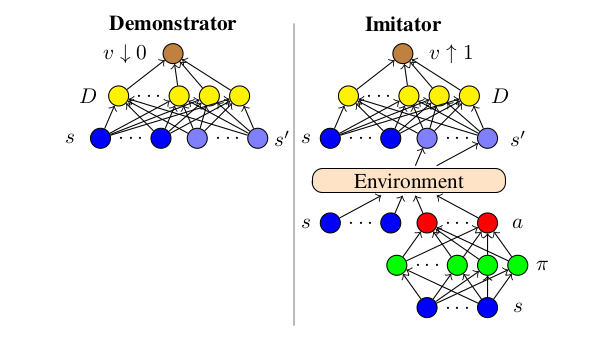
\includegraphics[height=7cm,page=1]{../img/GAN.png}
    \caption{GAN uzbūves piemērs. Augšējais tīkls --- diskriminators --- cenšas atšķirt eksperta demonstrācijas no ģeneratora radītām trajektorijām \cite{torabi2018generative}}
\end{figure}

Ģeneratīvie pretinieku tīkli --- GAN, \textit{generative adversarial networks} --- ir neironu tīkli, kas apmācīti visai īpatnējā veidā. Tā vietā, lai optimizētu visu modeli vienam mērķim, tiek izdalīti divi elementi --- ģenerators un diskriminators --- ar pretējiem uzdevumiem. Diskriminators ir klasifikators, kas apmācīts atšķirt demonstrāciju kopas trajektorijas vai to elementus no visām pārējām. Ģenerators no sistēmas stāvokļiem vai novērojumiem ģenerē darbības tā, lai diskriminators nebūtu spējīgs atšķirt tās no parauga. Formāli aprakstīt veidu, kā līdz šāda modeļa piemērotībai nonākts, ir sarežģīti, tāpat --- pierādīt šāda optimizācijas procesa konverģenci. Taču intuitīvi diezgan skaidrs, ka pēc sekmīgas abu modeļu apmācības būs iegūta stratēģija, kas tuvu aproksimē ievades datu sadalījumu.



\subsubsection{Uzdevumu simboliska dekompozīcija}

Vēl viena metode atdarināšanas spēju uzlabošanai ir telpisku kustības trajektoriju pārvēršana simbolisku, diskrētu darbību virknē. Pamatideja ir tāda, ka vieglāk iemācīties robusti izpidlīt primitīvas kustības un tad šādu primitīvo kustību secību kāda uzdevuma izpildē, nekā no neliela demonstrācija skaita iemācīties katru uzdevumu pilnībā no jauna. Šī arī nebūt nav jauna ideja --- izteikta jau 1980os un 1990os gados \cite{muench1994robot}. Jau 2002. gadā veikti pētījumi par algoritmiem, kas ļauj aproksimēt trajektorijas elementus ar autonomu, nelineāru diferenciālvienādojumu sistēmām \cite{ijspeert2002movement} un iemācīt pietiekami sarežģītas kustības --- piemēram, tenisa bumbas sišanu --- ar samērā nedaudziem piemēriem (ap 20). Ap to pašu laiku piedāvātas arī pieejas šādu primitīvu kustību kombinēšanai \cite{schaal2003computational}, kur mašīnmācīšanās lietojums attiecināts ne tikai uz atsevišķajiem trajektorijas primitīviem, bet arī uz katrai demonstrācijai atbilstošas to secības meklēšanu.

Pirms nesenā ļoti lielu neironu tīklu modeļu popularitātes uzplaukuma, šķiet, tieši simboliskās dekompozīcijas metodes bijušas starp perspektīvākajām. Robotikas literatūrā pirms 2010. gada \cite{billard2008handbook} gari un plaši rakstīts par šādiem paņēmieniem, taču pēdējos gados šī popularitāte varētu būt sarukusi. Jebkurā gadījumā, aktīva pētniecība nozarē vēl joprojām notiek, it sevišķi pielietojumiem, kur robots tiek mācīts ar kinestētiskām metodēm. Piemēram, ``\textit{A Framework of Hybrid Force/Motion Skills Learning for Robots}'' \cite{wang2020framework}, kas publicēts 2020. gadā, šāda pieeja tiek veiksmīgi izmantota uzdevumiem, kur svarīga ne tikai telpiskā trajektorija, bet arī uz apkārtējo vidi izdarīto spēku profils (piemēram, galda tīrīšanā).


\subsection{Novērojumu iegūšana, interpretācija, papildināšana}

Pat ja demonmstrācijas ir iespājams ļoti precīzi atdarināt, praksē paveras jauna problēma --- ne vienmēr iespējams tiešā veidā iegūt pietiekami labus paraugus no instruktoriem. Ja novērojums $o_t$ ir netiešs --- iegūts formā, kas neatbilst robota vadības algoritmam nepieciešamajam sistēmas konfigurācijas aprakstam --- to nepieciešams pārveidot. Turklāt, darbojoties ar netiešiem novērojumiem, bieži vien tiešā veidā iespējams atjaunot tikai stāvokļu $s_t$ laikrindu --- darbības $a_t$ paliek nezināmas.

Strādājot apstākļos, kur vienkārši analītiski modeļi ar labu precizitāti var paredzēt stāvokļa atribūtus un sakarības starp tiem, šī atšķirība var nebūt īpaši svarīga. Piemēram, darbojoties ar robotu, kas nav sevišķi smagi noslogots un kura kontroles sistēma spēj bez lielām novirzēm atdarināt no tās prasīto kinemātiku, nav daudz sarežģītāk darboties ar novērojumiem, kuros zināmi tikai šie kinemātiskie atribūti. Tas varbūt pat ir vienkāršāk, nekā izmantot smalkāku konfigurācijas aprakstu, kur pieejami arī visi dinamikas atribūti. 

Taču daudziem potenciāli ļoti noderīgiem lietojumiem galvenais šķērslis apmācībai var būt tieši derīgu treniņa datu kopu iegūšana no nepilnīgiem novērojumiem. Problēmas var sagādāt demonstrāciju ģenerēšana ar citādas ģeometrijas instruktoru (piemēram, cil-vēku), citu objektu sarežģītu un iepriekš nezināmu konfigurāciju modelēšana (manipulē-jamo objektu novietojums, orientācija, u.t.t.), trajektoriju automātiska iegūšana no datu kopām, kas nav tiešā veidā paredzētas šim mērķim (video ieraksti). Tāpat jāparvar zināmi izaicinājumi, lai datus varētu ģenerēt ar netiešām metodēm --- piemēram, attālinātu vadību vai virtuālās realitātes simulācijām.

\subsubsection{Nezināmas darbības}

Pētījumos, kuru galvenā būtība ir dažādu veidu pārveidojumi ar kinemātiskiem vai dinamiskiem trajektoriju datiem, varētu teikt, ka uzsvars ir uz kinestētiskajiem mācīšanās aspektiem. Ja iepriekšējā nodaļā aplūkoto eksperimentu veicēji pārsvarā pieņēmuši, ka pieejami pareizi formatēti dati, kuros novērojums ir cieši sakarīgs ar robota vadībai svarīgiem sistēmas atribūtiem un zināmas katrā trajektorijas solī veiktās darbības, tad šajā tiek apskatīti gadījumi, kad šie dati ir kādā ziņā nepietiekami vai pārveidoti.

Pirmais sarežģījums, ko varētu ieviest, ir darbību trūkums demonstrācijās. Ar to jāsastopas ļoti daudzos uzdevumos --- no nemarķētiem datiem var kā nebūt iegūt, piemēram, robota gala efektora pozīciju un rotāciju, taču nekas nav zināms par tā locītavu lenķiskajiem paātrinājumiem. Lai varētu izmantot jau zināmos atdarinošās mācīšanās algoritmus, rodas nepieciešamība uzminēt attiecīgās darbības, kas rezultē pārejā no viena stāvokļa uz nākamo.

``\textit{Behavioral Cloning from Observation}'' \cite{torabi2018behavioral} (2018) ir viena šāda metode. Tās mērķis ir realizēt jau aprakstīto uzvedības klonēšanas algoritmu laikrindu datiem, kuros pieejami tikai novērojumi. Lai to panāktu, tiek ieviests papildus modelis, tikai šoreiz nevis stratēģijas, bet gan paša robota (vai cita aģenta) dinamikas aproksimēšanai.

Nedaudz vienkāršojot tad algoritma soļi ir sekojoši:

\begin{enumerate}
    \item doto trajektoriju kopu pārveido formā $\mathcal{T}_{dem}=\lbrace (s_t, s_{t+1}) \rbrace$, kas ir pārejas starp stāvokļiem;
    \item stratēģija $\pi_{\theta}$ un sistēmas dinamikas modelis $M_{\phi}(a \vert s,s')=P(a \vert s, s')$ tiek nejauši inicializēti;
    \item ģenerē trajektorijas ar $\pi_{\theta}$, pievieno trajektorijas elementus kopai $\mathcal{T}=\lbrace (s_t, a_t, s_{t+1}) \rbrace$;
    \item apmāca $M_{\phi}(a \vert s, s')$ uz $\mathcal{T}$;
    \item trenē $\pi_{\theta}$ uz $\lbrace (s_t, \operatorname*{argmax}\limits_a M_{\phi}(a \vert s, s'), s')\vert (s, s') \in \mathcal{T}_{dem} \rbrace$
    \item atkārto soļus 3-5 līdz sasniegti pieņemami rezultāti
\end{enumerate}

Redzams, ka pakāpeniski tiek iegūts dinamikas modelis, kas pareizi paredz pārejas funkcijas slēpto darbības parametru, un, tāpat kā parastajā gadījumā, tiek apmācīta atbilstoša stratēģija. Interesanti arī, ka šajā situācijā potenciāli nedaudz lielāks uzsvars ir tieši uz nākamo novērojumu laikrindā, nevis izvēlēto darbību --- pie $s$, $\pi_{\theta}$ iemācās paredzēt \textit{s' sasniegšanai labāko darbību}, nevis vienkārši atkārtot pašu darbību bez konteksta, tātad savā ziņā sistēmas dinamika un vēlamais rezultāts tiek ņemti vērā. Rezultātos autori salīdzina šo metodi ar citām, kas izmanto arī darbību datus no demonstrācijām, un konstatē, ka šis algoritms pat strādā labāk nekā tādas, ja tiek vērtēts pēc nepieciešamo demonstrācijas trajektoriju vai simulācijas iterāciju skaita.

Iepriekšējā apakšnodaļā 2. attēls ir no ``\textit{Generative Adversarial Imitation from Observation}'' \cite{torabi2018behavioral} (2018), kas turpina darboties tajā pašā virzienā, tikai šoreiz ar GAN modeļa palīdzību. Tā vietā, lai modelētu sistēmas dinamiku, diskriminators klasificē trajektoriju laikrindās sastopamās stāvokļu pārejas $(s, s')$ pēc tā, vai tās būtu sastopamas demonstrācijā, bet ģenerators (kas reizē ir arī stratēģija $\pi_{\theta}$) tiek trenēts, lai tā izvēlēto darbību rezultātā iegūtās stāvokļu pārejas $s=T(s,a)$ nebūtu atšķiramas no piemēriem.

\subsubsection{Trajektorijas dinamikas atdarināšana, vispārināšana}

Cita veida problēma, kas arī prasa korekciju ieviešanu, ir atdarināšana sistēmām ar mainīgu dinamiku. Robotiem izmantojot ``\textit{lead-through}'' programmēšanas metodi, kustības tiek programmētas bez slodzes un, iespējams, neievērojot ātrumu --- zināma tikai daļēja sistēmas kinemātika. Ja var paredzēt, ka pēc tam ekspluatācijā atšķirsies robotu slogojošie spēki un griezes momenti, tad var meklēt veidus, kā šīs novirzes treniņa datu ieguves procesā kompensēt. ``\textit{Online Movement Adaptation based on Previous Sensor Experiences}'' \cite{pastor2011online} (2011) paredz jau iepriekš aprasktīto simboliskās dekompozīcijas modeļu papildināšanu ar korekcijām reālā laikā, izmantojot atgriezenisko saiti ar gan paša robota iekšējiem devējiem, gan ārējiem sensoriem. 

Pētījumos, kas nodarbojas ar simbolisko dekompozīciju, bieži vien tiek aprakstīti visai sarežģīti un tieši robotu dinamikai specifiski matemātiskie modeļi. Taču vienkāršoti procesu var aprakstīt sekojoši: kustības rakstorojošie diferenciālvienādojumu modeļi tiek iegūti, robotu manuāli vai citādi pārvietojot. Tad kustība tiek veikta ar pareizu kinemā-tiku (ātrumiem, paātrinājumiem), bet bez papildu slodzes. Tiek ierakstīti sensoru novēro-jumi un veidoti kustībai atbilstoši modeļi, kas paredz šos raksturlielumus trajektorijas gaitā. Autoru vārdiem --- robots iemācās, kā kustībai vajadzētu ``justies''. Tad reāli ekspluatācijā var sekot līdzi nobīdēm no normas un ar klasiskās kontroles teorijas metodēm veikt korekcijas.

Nodarbojoties ar ļoti sarežģītiem uzdevumiem --- piemēram, salikšanas procesiem --- mēģināt vadīt robotu cauri visiem iespējamiem detaļu savstarpējiem stāvokļiem var būt neiespējami. Ja var iegūt demonstrācijas kādā citā, vieglāk realizējamā veidā un izstrādāt vispārīgu metodi, kā tos atdarināt neatkarīgi no robota uzbūves, rodas iespējas automatizēt arī šādus procesus. ``\textit{Contact Skill Imitation Learning for Robot-Independent Assembly Programming}'' \cite{scherzinger2019contact} (2019) realizē šādu procedūru, izmantojot divus būtiskus elementus:

\begin{enumerate}
    \item \textit{forward dynamics compliance control} --- robota vadības algoritmu, kurā tiek kontrolēti uz efektoru iedarbojošos spēku un griezes momentu vektori, nevis izpildelementu pozīcija \cite{scherzinger2017forward};
    \item rekurentos neironu tīklus laikrindas nākamā elementa paredzēšanai --- t.i., tīklus, kuru ievadē parādās iepriekšējā laika soļa izvades vektors no tā paša modeļa;
\end{enumerate}

Demonstrāciju iegūšanai cilvēks simulācijas vidē ar datorpeles palīdzību veic salikšanas procesu, izmantojot tikai vizuālo uztveri un intuitīvu izpratni par sadursmju dinamiku. Novērojumus veido manipulējamā objekta masas centrā reģistrēto griezes momentu un spēku vektori. Stratēģija --- rekurentais neironu tīkls --- $\pi_{\theta}$ tiek apmācīta paredzēt nākamo spēku/momentu vektoru laikrindā, un tas tiek izmantots robota kontrolei ar minēto vadības algoritmu.

\subsubsection{Demonstrācijas no cilvēka darbībām}

Ja nepieciešams ātri un lēti radīt treniņa datu kopas apmācības procesiem --- kā tas noteikti būtu jebkurai praktiski izmantojamai robotu programmēšanas sistēmai --- svarīgi radīt cilvēkam draudzīgu saskarni. Tā vietā lai programmētu robota trajektoriju ar tradicionālām metodēm, ir veikti mēģinājumi attīstīt paņēmienus, kas ļautu dabiski ierakstīt cilvēka izpildītas kustības un izteikt tās formā, ko var izmantot robota apmācībai. Viens no virzieniem, kurā veikta izpēte, ir tieša fiziskās kinemātikas ierakstīšana un pārveidošana --- ``\textit{Imitation learning in industrial robots: a kinematics based trajectory generation framework}'' \cite{jha2017imitation} (2017) ir ilustratīvs piemērs. Tiek izmantota \textit{Microsoft Kinect} --- savulaik populāra videospēļu vadībai paredzēta kustību uztveres ierīce, kas spēj ierakstīt kāda objekta kustību aprakstošu punktu virkni telpā --- lai ierakstītu cilvēka kustības. Tad ar analītiskām metodēm tiek veikta trajektoriju interpolācija, grupēšana ar klasterizācijas algoritmu, un izpildē vēlamo trajektoriju iegūst ar tuvāko kaimiņu metodēm.

Lai mazinātu atšķirības starp cilvēkam un robotam pieejamām novērojumu un darbību telpām, var izmantot virtuālo realitāti --- gan simulācijās, gan robota tālvadībai. ``\textit{Deep imitation learning for complex manipulation tasks from virtual reality teleoperation}'' \cite{zhang2018deep} (2018) ir aprakstīta fiziska robota tālvadības sistēma, kas robota novēroto vidi pārveido sintētiskā telpā, kur cilvēks var ar manipulatoru palīdzību intuitīvi vadīt robota kustības. Šis uzdevums nav gluži triviāls, jo jāpārvar atšķirības starp, piemēram, robota kameras un cilvēka galvas kustību ātrumu, lai neradītu diskomfortu lietotājam. Tādējādi iegūta demonstrāciju datu kopa, kas sastāv no attēliem un telpiskiem dziļumiem, ko arī tālāk var izmantot konvolūciju neironu tīklā, lai realizētu uzvedības klonēšanu.

\subsubsection{Video demonstrācijas, perspektīvu pārbīde}

Ļoti plašas iespējas demonstrāciju iegūšanai pavērtu spēja tās iegūt no video datiem un izmantot šādas ``redzes'' sistēmas arī tiešā vadības uzdevuma risināšanai. Izrādās, ka daži no jau iepriekš aplūkotajiem algoritmiem ir pietiekami vispārīgi, lai tos varētu pielāgot šim uzdevumam. Piemēram, GAN no novērojumiem \cite{torabi2018generative} ir ļoti robusts attiecībā pret ievades datu formu un saturu, ja vien tajos ir iespējams pietiekami labi atšķirt demonstrāciju no citām trajektorijām. Tāpat kā gadījumā, kad strādā ar kinemātiku aprakstošiem stāvokļiem, GAN vienkārši tiek apmācīts diskriminēt/ģenerēt trajektoriju vizuā-lās reprezentācijas, ar samērā labiem rezultātiem.


Brīdī, kad vairs netiek izmantoti robota konfigurāciju aprakstoši novērojumi, rodas jauna problēma --- iegūtie novērojumi ir atkarīgi no izmantotās perspektīvas, kas vispārīgā gadījumā var arī nesakrist ar robota vadības algoritmu ievades datus ģenerējošo. ``\textit{Imitation from observation: Learning to imitate behaviors from raw video via context translation}'' \cite{liu2018imitation} (2018) risina šo atšķirīgo kontekstu sarežģījumu un iegūtu modeli izmanto arī rezultātu uzlabošanai vispār. Pieņemot, ka trajektorijai atbilstošie novērojumi tiek iegūti no dažādām perspektīvām telpā, vispirms tiek apmācīts enkodera-dekodera tipa neironu tīkls, kas iegūst novērojumu vektoriālas reprezentācijas, ko pēc tam iespējams dekodēt par tai pašai sistēmas konfigurācijai atbilstošu novērojumu no jebkuras perspektīvas. Tas ļauj ne tikai tiešā veidā ``tulkot'' novērojumus no vienas kameras uz citu, bet arī izmantot iegūtās kodētās reprezentācijas Eiklīda distanci no demonstrāciju trajektoriju soļiem atbilstošajām kā atalgojuma funkciju stimulētās mašīnmācīšanās algoritmam. Arī intuitīvi skaidrs, ka modelis, kas spēs atjaunot situācijas attēlu kādā perspektīvā, ja zināmi tikai no citas perspektīvas gūtie attēli, kaut kādā ziņā sevī ietver visus nozīmīgos konfigurācijas atribūtus.

\subsubsection{Datu sintēze, telpiski modeļi}

\begin{figure}[t!]
    \centering
    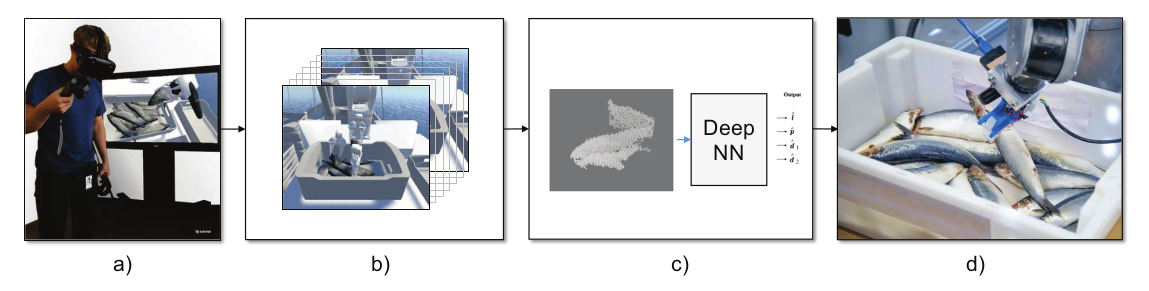
\includegraphics[width=16cm]{../img/fish.png}
    \caption{Zivs satveršanas modeļa apmācība: a) cilvēka radīto demonstrāciju iegūšana; b) datu kopas sintētiska pavairošana; c) telpiska konvolūciju neironu tīkla apmācība; d) veiksmīga zivs satveršana realitātē. \cite{dyrstad2018teaching}}
\end{figure}

Daudzi uzdevumi, kam tiek izmantoti roboti, sevī ietver manipulāciju ar citiem objektiem, kuru telpisko novietojumu un citus atribūtus ne viemēr viegli iegūt, un nākas paļauties uz netiešiem novērojumiem, ko sagādā, piemēram, tehniskās redzes sistēmas. Ja objekti ir paredzamā orientācijā un regulāras formas, no šīs problēmas parasti iespējams izvairīties, taču vēl joprojām daudzi pārvietošanas un pozicionēšanas procesi tiek veikti ar cilvēka roku darbu.

``\textit{Teaching a robot to grasp real fish by imitation learning from a human supervisor in virtual reality}'' \cite{dyrstad2018teaching} ir visnotaļ interesants vairāk praktisks projekts, kura ietvaros izstrādāts modelis zivju satveršanas uzdevumam. Šo rakstu irr vērts nedaudz sīkāk aplūkot, jo problemātika ir radniecīga darba mērķī formulētajam uzdevumam --- industriālā robota darbības ar neregulāras formas objektiem. Tajā robotam ir jāspēj no kastes, kurā atrodas vairākas zivis, satvert un pārvietot vienu. Zivs ir slidens objekts, kas padevīgs satveršanai ar robota efektoru tikai ļoti ierobežotā iespējamo kontakta konfigurāciju apakškopā, tāpēc no praktiskas realizācijas viedokļa projekts ir visai ambiciozs. 

Risinājuma pamatā ir trīs idejas:

\begin{enumerate}
    \item zivs pozīcijai un orientācijai piemērota satveršanas punkta un lenķa paredzēšana no ar telpisko kameru gūtiem telpiskiem punktu mākoņa datiem. Tam pielieto konvolūciju neironu tīklu --- izmantojot vispārinātas metodes, kas sākumā izmantotas divdimensionāla attēlu klasifikācijai;
    \item demonstrāciju ievākšana virtuālās realitātes vidē, kas ļauj cilvēkam viegli un dabiski ģenerēt satvērienus;
    \item datu kopas sintētiska pavairošana.
\end{enumerate}

Novērojumi gūti, cilvēkam VR vidē brīvā veidā satverot zivis dažādos veidos. Lai viennozīmīgi aprakstītu katru iespējamo satvērumu, izmantoti trīs vektori --- pozīcija (punkta), garenās ass orientācija un rotācija ap to.  Pēc tam ģenerēts liels skaits zivju izvietojuma konfigurāciju. Lai sintētiskie dati būtu lietojami, nepieciešams nodrošināt, ka satvēruma matrica tiek koriģēta atbilstoši zivs izliekumam, novietojumam un orientācijai. Katrā sagatavotajā sistēmas konfigurācijā katrai zivij sākumā piešķirti visi iespējamie satvēruma vektori, no kuriem atsijāti visi, kas kolīziju dēļ nav sasniedzami. Šie dati tad izmantoti 3-dimensionālā konvolūciju neironu tīkla apmācībai --- simulatorā ģenerēti ainai atbilstoši telpiskie attēli, modelis apmācīts kā tipisks klasifikators. Rezultātā konstatēts, ka aptuveni 74\% izdarīto satveršanas mēģinājumu bijuši sekmīgi.

\subsection{Atdarināšana un adaptācija, vispārināšana}

Ja pieejamas demonstrācijas no eksperta, to atdarināšana tiešā veidā varbūt ir pirmais solis noderīgu stratēģiju iegūšanā, taču nebūt ne vienīgais, ko iespējams darīt. Līdz šim aplūkotas metodes, kas izrāda zināmu adaptācijas pakāpi, lai precīzāk un robustāk imitētu paraugus, taču vienmēr izdarīts pieņēmums, ka instruktors kādā ziņā optimāli izpildījis uzdevumu. Turklāt visos gadījumos, lai apmācītu sistēmu izpildīt jaunu uzdevumu, nepieciešams veikt intensīvu treniņu ar cilvēka starpniecību. 

Šajā apakšnodaļā aprakstīti pētījumi, kuros meklēti veidi, kā apvienot atdarināšanu ar adaptāciju, lai vispārinātu demonstrācijās ietverto informāciju, atvieglotu jaunu uzdevumu programmēšanas procesu vai pārspētu instruktoru sasniegto rezultātu kvalitātē. Lai gan mēģinājumi darboties šajā jomā nav nekas jauns --- var atrast senākus pētījumus, kuros, piemēram, izmantotas sarežģītas un tieši robotikas mērķiem specifiskas simboliskās dekompozīcijas metodes \cite{pastor2011skill} --- uzsvars šeit tiek likts uz nesenākām un vispārīgākām metodēm, kas attīstītas jau pašreizējā neironu tīklu uzplaukuma periodā.

\subsubsection{Neoptimālu demonstrāciju uzlabošana}

Varētu sacīt, ka jau pati atdarinošās mācīšanās pamatnostādne --- apgūt stratēģiju problēmas risināšanai, pēc iespējas tuvāk sekojot kādai demonstrāciju kopai --- sevī ietver pieņēmumu par demonstrācijas optimalitāti. Taču izrādās, ka iespējams pašu treniņa datu kopu izmantot, lai gūtu informāciju par to, ko instruktors patiesi vēlējies sasniegt, un attiecīgi optimizēt modeli šī slēptā mērķa sasniegšanai.

``\textit{Extrapolating beyond suboptimal demonstrations via inverse reinforcement learning from observations}'' \cite{brown2019extrapolating} (2019) izmanto jau iepriekš aprakstīto inversās stimulētās mācīšanās algoritmu saimi par pamatu jaunai metodei. Tā vietā, lai atrastu atalgojuma funkciju, kas pamato demonstrāciju kopas trajektorijas $\tau$, tiek meklēta tāda, kas skaidro to \textit{sakārtojumu}. Tāpēc nepieciešāms datu kopu papildināt ar kārtojumu $\prec$, lai

\begin{equation}
    \tau_i \prec \tau_j \Rightarrow \sum_{s_t \in \tau_i}R(s) \leq \sum_{s_t \in \tau_j}R(s)
\end{equation}

Protams, kārtojums var arī nebūt ideāls --- trajektoriju vērtējums var būt subjektīvs vai trokšņains, ja nav zināma īstā atalgojuma funkcija, tāpēc jārēķinās ar kļūdainu pāru attiecību pastāvēšanas iespējamību ar kļūdas varbūtību $\epsilon$

\begin{equation}
    \exists \epsilon > 0 : \tau_i \prec \tau_j \Rightarrow P\left(\sum_{s_t \in \tau_i}R(s) \leq \sum_{s_t \in \tau_j}R(s)\right) \geq 1 - \epsilon
\end{equation}

Ja kārtojums ir pieejams, radoši nosauktais \textit{Trajectory-ranked Reward EXtrapolation} jeb T-REX algoritms darbojas divos soļos:

\begin{enumerate}
    \item izmantojot demonstrāciju datus, tiek apmācīta nezināmās atalgojuma funkcijas $R(s)$ aproksimācija $r_{\phi}(s)$ --- parametrisks modelis, konkrēti neironu tīkls;
    \item tāpat kā IRL gadījumā, rekonstruētā atalgojuma funkcija tiek izmantota, lai apmā-cītu stratēģiju $\pi_{\theta}$ ar stimulētās mašīnmācīšanās metodēm.
\end{enumerate}

Eksperimentāli pārbaudīts, ka piemēros, kur zināmas demonstrācijām atbilstošās īstās atalgojuma funkcijas un kļūdas varbūtība saglabājas zem 15\%, rekonstruētā atalgojuma funkcija $r_{\phi}$ daudzos gadījumos labi aproksimē īsto. Turklāt, ja izmantotās demonstrācijas nav optimālas, iegūtā stratēģija $\pi_{\theta}$ tās pārspēj.

\subsubsection{Demonstrācija --- sākumpunkts apmācību procesam}

Atšķirībā no IRL un augstāk aprakstītā T-REX, ir iespējams uz atdarinošās un stimulētās mācīšanās kombināciju skatīties arī no otras puses --- nevis izmantot stimulētās metodes, lai realizētu atdarināšanu, bet gan izmantot demonstrācijas, lai uzlabotu parasto stimulētās mašīnmācīšanās procesu ar zināmu atalgojuma funkciju.

``\textit{Deep Q-learning from demonstrations}'' \cite{hester2018deep} (2018) piedāvā vispārīgu metodi stimu-lētās mācīšanās procesa inicializācijai ar demonstrāciju datu kopas palīdzību. Šādu pieeju motivē viens no lielākajiem klupšanas akmeņiem RL algoritmu apmācībā --- ja atalgojuma funkcijas nenulles vērtības konfigurāciju telpā ir stipri retinātas, kā tas ļoti bieži ir arī dažādos robotikas uzdevumos, tad, praktiski apmācot stratēģiju izpildīt tai uzdoto uzdevumu, nepieciešams ļoti liels skaits treniņa soļu --- lai šo telpu apstaigātu, atrastu vēlamos rezultātus un optimizētu trajektoriju caur tai.

Q-mācīšanās gadījumā stratēģiju var uzdot formā $\pi^{\epsilon Q_{\theta}}$, kur

\begin{equation}
    T(s,a) = P(s') \rightarrow Q_{\theta}(s,a) \sim \mathbb{E}[v(s')] 
\end{equation}

jeb modelis $Q_{\theta}$ aproksimē kopējā atalgojuma sadalījumu pār iespējamām darbībām (jeb nākamo stāvokļu vērtības), un attiecīgi izvēlas vienu pēc ``$\epsilon$-alkatīgas'' stratēģijas

\begin{equation}
    a = \operatorname*{argmax}_a Q(s,a) \text{ ar varbūtību } 1-\epsilon; \text{ nejauši izvēlēta citādi}
\end{equation}

Demonstrācijas tad tiek izmantotas, lai apmācītu $Q_{\theta}$ vēl pirms notiek jebkāda modeļa mijiedarbība ar vidi, un attiecīgi tas jau uzreiz darbojas daudz kvalitatīvāk nekā nejauši inicializēts modelis. Rezultāti liecina, ka jau sākotnējās iterācijās šāds algoritms var darboties visai labi, kas paver iespējas to izmantot situācijās, kad nav iespējams veikt apmācību simulācijas vidē, bet ir pieejami demonstrāciju dati. Robotikas kontekstā tas nozīmē, ka, ja jāveic apmācība uz fiziska robota, modeļa sagatavošana ar atdarināšanu varētu būt visai noderīgs paņēmiens.


\subsubsection{Tūlītēja trajektoriju atdarināšana}

Daudzas līdz šim aplūkotās atdarinošās metodes darbojas ar pieņēmumu, ka mērķis ir no demonstrāciju datu kopas iegūt modeli, kas pēc apmācības spēj izpildīt vienu uzdevumu, un attiecīgi treniņa algoritms neparedz iespēju bez papildus iterācijām atdarināt iepriekš neredzētas demonstrācijas --- tipiski pieejams tikai pašreizējais sistēmas stāvoklis ievadē un vēlamā darbība izvadē.

Salīdzinot ar bioloģiskām sistēmām, uzreiz ir skaidrs, ka šādi procesi nekad nespēs izdarīt cilvēkam šķietami pašsaprotamo --- novērot darbību un uzreiz to atkārtot bez liela skaita treniņa iterāciju. Lai būtu iespējams sasniegt šādu rezultātu, ir nepieciešams nevis modelis, kas ar paraugiem ticis optimizēts vienas stratēģijas atdarināšanai, bet gan tāds, kas vispārina pašu atdarināšanas procesu --- ievadē sistēmas pašreizējais stāvoklis tiek apvienots ar demonstrāciju, lai iegūtu vēlamo darbību. 

``\textit{One-Shot Imitation Learning}'' \cite{duan2017one} (2017) šādu rezultātu sasniedz, apmācot sarež-ģītas uzbūves modeli, kas apmācīts no vienas demonstrācijas paredzēt citas vispārīgā veidā --- tā ievades vektors satur veselu treniņa kopas trajektoriju. Modelis tiek apmācīts uzreiz veselai līdzīgu uzdevumu kopai, nevis tikai vienam konkrētam.

Konkrēti, pētītā uzdevumu saime ir kuba formas detaļu kraušana vienai uz otras ar robotu. Novērojumu ģenerēšanas un interpretēšans problēmas gan tiek apietas, jo sistēmas stāvokli raksturojošie vektori satur gan robota iekšējo konfigurāciju, gan detaļu relatīvās pozīcijas attiecībā pret robota efektoru. Tad, izmantojot konvolūciju un uzmanības mehānismus, dažādu garumu trajektoriju laikrindas tiek reduētas uz vienu sistēmas stā-vokļa vektoru, kas paredz piemērotāko darbību attiecībā pret doto demonstrāciju un momentāno sistēmas stāvokli.

\subsubsection{Nestrukturētas demonstrācijas, plānu veidošana no galamērķiem}

Droši vien lielākā atkāpe no ``klasiskā'' atdarinošā mašīnmācīšanās uzdevuma ir tajos pētījumos, kur tiek atmests pieņēmums, ka ir dotas diskrētas parauga trajektorijas ar zināmu uzdevumu. Tā vietā pat pārraudzītā trajektoriju marķēšanas stadija tiek automatizēta un atstāta apmācības algoritma pārziņā. Tā vietā var novērot, ka, ja mērķis ir iemācīties modeli, kas spēj vispārīgi atrast ceļu no vienas sistēmas konfigurācijas uz citu, pietiek atrast trajektorijas, kas iet caur abām. ``\textit{Learning Latent Plans from Play}'' \cite{lynch2020learning} (2019) ierosina demonstrāciju strukturētas ievākšanas vietā izmantot cilvēka dabisko tendenci spēlēties ar dažādiem objektiem, lai virtuālās realitātes vidē ģenerētu demonstrāciju kopas. Sistēma šajā gadījumā ir virtuālā realitātē modelēta vide, bet pieejamie novērojumi --- robota iekšējā konfigurācija un simulēti attēli.

Tiek konstatēts, ka, pilnīgi nejauši ģenerējot trajektorijas, paies visnotaļ ievērojams laiks, līdz tiks apstaigāts pietiekami plašs konfigurāciju telpas reģions, lai gūtu labas trajektorijas starp jebkuriem punktiem tajās. Atšķirībā no nejauša procesa, cilvēks jau nāk ar sagatavotu izpratni par tāda tipa uzdevumu risināšanas elementiem, kas pēc tam varētu būt interesanti citiem. Brīvi pētot dažādās simulācijas vidē pieejamās iespējas, tiks dabiski izmantotas priekšzināšanas par dažādām fizikālām sakarībām starp objektiem un to mijiedarbību --- piemēram, rokturu satveršanu, lai atvērtu un aizvērtu durvis, pogu nospiešanu, objektu satveršanu un pacelšanu.

Lai no šādas nestrukturētas informācijas iegūtu praktiski izmantojamas stratēģijas, nepieciešams papildināt stratēģijas formālismu ar mērķa jēdzienu --- ne vairs vienkārši atrodot katram stāvoklim piekārtotu $\pi(s)$, bet gan parametrizētu pēc vēlamā beigu stā-vokļa (\textit{goal}) --- $\pi(s,s_{g})$. Ja pieejamas trajektoriju laikrindas formā $s_1, s_2, ..., s_n$, nav grūti pamanīt, ka jebkura apakšvirkne veido sākuma-gala stāvokļu pāri ar visām to starpā esošajām pārejām.

Tiek piedāvāti divi dažādi modeļu šabloni un apmācības algoritmi, kas spētu iegūt reālas stratēģijas no nestrukturētu datu kopas. Vienkāršojot --- ignorējot sistēmas stā-vokļa reprezentāciju kodēšanas detaļas --- pirmo var aprakstīt samērā vienkārši. Modelis $\pi_{\theta}(s,s_g)$ saņem ievadē pašreizējo un vēlamo stāvokli, un paredz nepieciešamo darbību. Kā šablons tiek izmantots rekurentais neironu tīkls, treniņa datus veido trajektorijas --- pēdējais trajektorijas stāvoklis kļūst par $s_g$, un $\pi_{\theta}$ optimizē, lai katram $(s_t, a_t, s_g)$ būtu $\pi_{\theta}(s_t, s_g) \approx a_t$. Taču pastāv problēma --- var pastāvēt dažādas trajektorijas starp jebkuriem $s, s_g$, kas draud apgrūtināt mācīšanās procesu.

Otrs, sarežģītākais modelis apkaro šo parādību, modelējot plāna jēdzienu --- tiek pieņemts, ka katrai trajektorijai $\tau$ var piekārtot rīcības plānu, visiem iespējamiem rīcības plāniem pastāv vektoriālas reprezentācijas $z$, un vieglāk ir vispirms paredzēt atbilstošāko plānu, pēc tam --- piemeklēt tam viennozīmīgi piekārtotu trajektoriju. Modelis tad sastāv no trim daļām:

\begin{enumerate}
    \item plānu enkodera $q_{\phi}(z \vert \tau)$, kas izsaka trajektorijas ar matemātisko cerību un standartnovirzi vektoriem $\mu_{\phi}, \sigma_{\phi} = q_{\phi}(\tau)$;
    \item plānu selektora $q_{\psi}(z \vert s, s_g)$, kas analoģiski paredz $\mu_{\psi}, \sigma_{\psi} = q_{\psi}(s, s_g)$ un iegūst no sadalījuma konkrētu vektoru $z$ diferencējamā veidā (pieskaitot vidējām vērtībām gadījuma lieluma reizinājumu ar standartnovirzi);
    \item dekodera $\pi_{\theta}(z, s, s_g)$, kas rekonstruē nepieciešamo darbību no plāna reprezentācijas, galamērķa un sistēmas momentānā stāvokļa.
\end{enumerate}

Divi varbūtību sadalījumi $q$ nepieciešami, jo optimizācijas procesā tiek minimizēta Kulbaka-Leiblera diverģence starp tiem --- ļaujot visu trajektoriju aizstāt ar tikai diviem tās punktiem. Otrs mērķa funkcijas faktors ir kļūda darbībā $a_t$. Tā kā visi slāņi ir diferencējami, viss modelis kopā veido vienu neironu tīklu, ko kopā arī apmāca uz trajektoriju apakšvirknēm. Stratēģija ir $\pi_{\theta}(q_{\psi}(s, s_g), s, s_g)$.

Tātad, lai programmētu robotu izpildīt kādu konkrētu uzdevumu, vairs nav nepieciešamas ne papildus treniņa iterācijas, ne demonstrācijas --- pietiek norādīt vēlamo sistēmas gala stāvokli, un stratēģija to pati sasniegs. Rezultātu sekcijā secināts, ka šāda mācīšanās spēj pārspēt klasisko uzvedības klonēšanas metodi 18 dažādiem uzdevumiem --- kaut gan otra izmantojusi demonstrācijas, kas speciāli sagatavotas katram. Turklāt, pateicoties faktam, ka modelis apgūst trajektorijas no katra konfigurāciju telpas punkta uz katru citu, tā ir ļoti robusta pret nobīdēm. Visbeidzot, ar dimensiju redukcijas metodēm aplūkojot iegūto rīcības plānu reprezentācijas telpu redzams, ka pēc cilvēkam saprotama mērķa līdzīgas darbības veido klasterus arī šajās projekcijās.

Interesants turpinājums šim pētījumam ir ``\textit{Language conditioned imitation learning over unstructured data}'' \cite{lynch2021language}, kur iegūtais rezultāts atkal pagriezts otrādi --- ja ir metode, kas spēj pati izdalīt uzdevumus un grupēt tos pēc būtības, tad apvienojot to ar sagatavotiem marķējumiem, var iegūt stratēģiju, kas vadāma ar šādiem marķējumiem. Konkrēti, ja daļai no trajektorijām tiek \textit{a posteriori} piekārtots dabiskā valodā izteikts mērķis, var apmācīt modeli, kas sasaista rīcības plānu reprezentācijas ar frāžu reprezen-tācijām --- ļaujot vadīt robotu ar jau iepriekš apmācītu valodas enkoderu ģenerētiem kodiem. Praktiski tas izpaužas tā, ka iespējams robotam dot pavisam dabiskas komandas, turklāt neatkarīgi no izvēlētajiem sinonīmiem un pat dažādās valodās.

Ar tīri atdarinošām metodēm iegūtas stratēģijas var nebūt optimālas, it sevišķi gadījumos, kad tiek prasīts sasniegt mērķi, kam nav sagatavota speciāla demonstrāciju datu kopa.`\textit{Relay policy learning: Solving long-horizon tasks via imitation and reinforcement learning}'' \cite{gupta2019relay} (2019) piedāvā apvienot nestrukturētas demonstrāciju datu kopas un galamērķus kā uzdevuma specifikāciju ar zināmu atalgojuma funkciju. Tā varētu iegūt labas inicializācijas apmācības procesiem, kas citādi būtu nepraktiski vai teju neiespējami ar vienkāršām konfigurāciju telpas pārstaigāšanas metodēm retināto atalgojuma vērtību dēļ.

Pamatā risinājumam ir hierarhiskā stimulētā mācīšanās --- tiek iegūta nevis viena stratēģija, bet divas. $\pi_{\theta}^h$ jeb augsta līmeņa stratēģija ievadē saņem pašreizējo sistēmas stāvokli $s$ un gala stāvokli $s_g$, bet tā vietā, lai izvadītu vēlamo darbību, rezultātā izdod lokālu mērķi $s_g^l$ --- argumentu zemākā līmeņa stratēģijai $\pi_{\phi}^l$. Otrā tad atkarībā no $s,s_g^l$ ģenerē vēlamo darbību vidē $a$. Apmācība tiek realizēta divos soļos:

\begin{enumerate}
    \item atdarināšana --- katrai no stratēģijām tiek sagatavota atsevišķa datu kopa, izmantojot ``slīdošā loga'' principu pār trajektorijām demonstrāciju datos. $\pi_{\theta}^h$ izvēlas plašāku logu $W_h$ un minimālo distanci līdz lokālajam mērķim $j$. Katram $s_t $ tad tiek izveidoti korteži $(s_t, a_t', s_g)$ kur $s_g \in \lbrace s_{t+1}, s_{t+2}, ..., s_{t+W_h} \rbrace$ bet $a_t' = s_{t+j}$. Zema līmeņa stratēģijai $\pi_{\phi}^l$ tad izvēlas īsāku logu $W_l$ un analoģiski katru tālāk logā esošo $s_{t+i}$ izmanto kā galamērķi $s_g^l$, lai izveidotu $(s_t, a_t, s_g^l)$. Šādi pārveidotos datus tad izmanto, lai apmācītu modeļus $\pi_{\theta}^h, \pi_{\phi}^l$ atdarināt datu kopu;
    \item uzlabošana --- izmantojot zināmu atalgojuma funkciju $r(s,a,s_g)$, realizē stimulēto mācīšanos. Iegūtās stratēģijas tiek darbinātas vidē, iegūtie dati tiek tāpat pārkārtoti un $\pi_{\theta}^h, \pi_{\phi}^l$ atkal tiek optimizēti, tikai šoreiz gradientu optimizācijas mērķa funkcija (\textit{loss}) tiek papildināta ar atalgojuma faktoru.
\end{enumerate}

Tiek iegūts algoritms, kas spēj no nestrukturētas datu kopas iemācīties, kā sasniegt patvaļīgus galamērķus, bet pēc tam --- uzlabot iegūtās stratēģijas ar stimulētās mācīšanās palīdzību. To parāda rezultāti --- dažādos uzdevumos šāda pieeja pārspēj iepriekš aprakstīto latento plānu pieeju \cite{lynch2020learning}, taču attiecīgi tai ir nepieciešama papildu patstāvīgas mācīšanās etaps.

\newpage
\section{Secinājumi}

Literatūras analīzē sniegts īss un nebūt ne pilnīgs --- vai vienlīdzīgi sadalīts --- līdz šim par atdarinošo mašīnmācīšanos veiktās pētnieciskās darbības pārskats. Jau izvēloties, par kurām tēmām rakstīts plašāk, par kurām --- mazāk detalizēti --- iespaidu uz darba saturu ir atstājusi motivējošās problēmas specifika. Tagad nepieciešams pie tās atgriezties un novērtēt, kas no visa nozarē pētītā un izgudrotā attiecas uz darba ievadā aprakstīto uzdevumu --- mešanas kustību iestrādāšanu atkritumu vai citu objektu pārvietošanā.

\subsection{Svarīgākās atziņas}

Tūlīt kļūst skaidrs, ka pašas vienkāršākās metodes --- klasiskā uzvedības klonēšana \cite{pomerleau1989alvinn} vai kādas tās tiešās korekcijas --- uzdevumam piemērotas nav. Tās darbojas gadī-jumos, kad demonstrāciju kopa labi nosedz visas iespējamās trajektorijas sistēmas konfigurāciju telpā, nav robustas pret nobīdēm, un jaunu trajektoriju programmēšana prasa apmācības procesa atkārtošanu. Problēmu grūti nostādīt formā, kur robotam vienkārši jāapgūst maksimāli precīzi atdarināt detalizētu un pilnībā aprakstošu demonstrāciju kopu. Vēl jāatzīst, ka metodes, kas ir ļoti specifiskas tieši robotikas uzdevumiem un prasa no algoritma izstrādātājiem pieņēmumus par uzdevuma struktūru --- t.i, pamatā risinājumi, kas nodarbojas ar simbolisko dekompozīciju \cite{ijspeert2002movement,schaal2003computational, wang2020framework,pastor2011online,pastor2011skill} --- nešķiet sevišķi perspektīvas, jo tās ir grūtāk attīstīt un vispārināt. Protams, no inženiertehniskā viedokļa tās varētu zināmos uzdevumos pārspēt vispārīgākas pieejas, tomēr ilgtermiņa pieredze rāda, ka dažādas lokālas priekšrocības mēdz izgaist, pieaugot daudzparametru neironu tīklu veiktspējai.

Runājot par novērojumiem, nozīmīgi šķiet tieši pētījumi, kas realizē demonstrāciju ievākšanu no cilvēka kustībām \cite{jha2017imitation,zhang2018deep} vai nu virtuālā, vai fiziskā telpā. Metienu izdarīšana ir intuitīvi labi trenēta taču analītiski sarežģīta procedūra. Ātra piemēru iegūšana varētu kalpot par pamatu rīkiem, ar ko praktisku sistēmu pielāgot tās apkārtējai videi darba zonā. Tāpat uzmanību vērts pievērst pētījumiem, kas izmanto telpiskus un video novērojumus kā arī datu kopas sintētisku pavairošanu \cite{dyrstad2018teaching}. Lai gan tiešā veidā kādu no tajos apraks-tītajiem algoritmiem droši vien neizdosies izmantot, ir vērts paturēt prātā metodes, ar ko trajektorijas padarītas noturīgākas pret novirzēm --- vai nu trenējot slēptu dinamikas modeli \cite{torabi2018behavioral}, vai arī izmantojot analītiskas kompensācijas \cite{pastor2011online}. Pastāv iespēja, ka būs nepieciešams izmantot novērojumus, kas iegūti no dažādām perspektīvām, tāpēc noderīgi varētu izrādīties arī perspektīvu pārneses paņēmieni \cite{liu2018imitation}.

Visbeidzot, no adaptīvo un imitējošo metožu kombinācijas virziena ļoti svarīgi šķiet rezultāti, kas gūti izstrādājot stratēģijas, kuras spēj pielāgoties dažādu demonstrāciju atdarināšanai \cite{duan2017one} vai dažādu galamērķu sasniegšanai bez papildus apmācības \cite{lynch2020learning,lynch2021language,gupta2019relay}. Tā kā ir iespējams diezgan skaidri definēt atalgojuma funkciju objekta iekrišanai pareizajā tvertnē, bet nonākšana līdz tai ar parastu stimulētās mācīšanās procesu ir ļoti apgrūtināta, risinājuma izstrādes gaitā var nākties izmantot arī atdarināšanu kā sākumpunktu pašmācībai \cite{hester2018deep}. 



\subsection{Plāns tālākai darbībai}

Apkopojot visu augstāk minēto, var ieskicēt risinājuma plānu uzdevumam. Lai apmācītu modeli, kas realizē metiena kustību ar jau satvertu neregulāras formas objektu, tiks darīts sekojošais:

\begin{enumerate}
    \item demonstrāciju ievākšana --- cilvēka veikti metieni fiziskā telpā vai VR tiks ierakstīti, iegūtas trajektorijas vai metienu raksturojoši parametri. Varētu veidot simulāciju un analītiski iegūt pareizus metiena parametrus, taču tas mazinātu rezultātu vispā-rīgumu --- taču atkarībā no pieejamā laika un resursiem, varētu gadīties, ka tā ir vienīgā praktiskā metode. Tāpat iespējams, ka katru metienu var reducēt uz objekta ātruma un lenķiskā ātruma vektoriem atlaišanas brīdī --- to, vai šādi pārveidojumi procesu atvieglos vai apgrūtinās, būs jānosaka praksē;
    \item datu kopas papildināšana --- iegūto demonstrāciju kopu varētu sintētiski pavairot, ja tiek veikta mesto objektu trajektoriju simulācija;
    \item atdarinoša modeļa apmācība --- jāizmanto modelis, kas parametrizēts pēc sasnie-dzamā galamērķa, lai būtu iespējams ātri un lēti pielāgot robotu darbam ar dažādi izvietotām tvertnēm;
    \item papildus optimizācija --- ja iespējams, ar nelielas un neoptimālas demonstrāciju kopas palīdzību apmācītu modeli var ievērojami uzlabot, papildus izmantojot stimu-lētās mācīšanās metodes. Atalgojuma funkciju šoreiz ir samērā viegli definēt (bet grūti sasniegt).
\end{enumerate}

Šobrīd grūti paredzēt, kādi rezultāti tiks sasniegti eksperimentālajā darbībā, kuri pieņēmumi būs izrādījušies patiesi, kuri --- aplami. Tāpat vēl pāragri spriest par konkrē-tiem tehniskiem izpildījumiem, jo tas ir ļoti atkarīgs no izmantotās datu kopas atribūtiem. Taču ir pamats ticēt, ka maģistra darba praktiskās daļas izpildījums iekļausies augstāk aprakstītā plāna ietvaros.

\newpage
\addcontentsline{toc}{section}{Atsauces}
\printbibliography[title=Atsauces]

\end{document}